% Full paper: Can an AC Battery Outperform the Conventional Two-Level Inverter?
% Build (from this folder):  latexmk -pdf PCIM_paper.tex
% (biber: see the build note in PCIM_synopsis.tex)
%
% Every figure and table with numbers is generated from the Python package in ../python:
%   python/venv/bin/python python/cycle_eval.py                 # cycle results + traces
%   python/venv/bin/python doc/figures/make_cycle_figures.py    # cycle_summary.pdf
%   python/venv/bin/python doc/figures/make_paper_maps.py       # figures/maps/<app>/*.png
%   python/venv/bin/python doc/figures/make_paper_assets.py     # figures/paper_*.pdf, tables/*.tex

\documentclass{PCIM-Abstract}

\usepackage[T1]{fontenc}
\usepackage[scaled=0.9]{inconsolata}
\usepackage{tikz}
\usetikzlibrary{positioning,calc,arrows.meta,shapes.geometric,fit,backgrounds}
\usepackage{booktabs}
\usepackage{array}
\usepackage{multirow}
\usepackage{amssymb}
\usepackage{bm}
\usepackage{listings}
\usepackage{xcolor}
\usepackage{longtable}
\usepackage{float}

\DeclareSIUnit\rpm{rpm}
\DeclareSIUnit\pp{pp}
\DeclareSIUnit\ohm{\ensuremath{\Omega}}

% code identifiers in a monospaced face (the class maps \ttfamily to sans serif)
\newcommand{\code}[1]{{\fontfamily{zi4}\selectfont\detokenize{#1}}}
\lstset{
  basicstyle=\fontfamily{zi4}\fontsize{8.5}{10.2}\selectfont,
  mathescape=true, columns=fullflexible, keepspaces=true,
  frame=single, framerule=0.3pt, rulecolor=\color{black!40},
  xleftmargin=2pt, xrightmargin=2pt, aboveskip=6pt, belowskip=4pt,
  numbers=left, numberstyle=\tiny\color{black!55}, numbersep=5pt,
  keywordstyle=\bfseries, morekeywords={for,each,if,else,while,return,do,end,then,and,or,in,break,continue,to,until,step,set,compute,solve},
  commentstyle=\color{black!55}, morecomment=[l]{//}
}
\renewcommand{\lstlistingname}{Alg.}
\crefname{lstlisting}{Alg.}{Algs.}
\Crefname{lstlisting}{Algorithm}{Algorithms}
\crefname{table}{Tab.}{Tabs.}
\Crefname{table}{Table}{Tables}
\crefname{section}{Sec.}{Secs.}
\Crefname{section}{Section}{Sections}
\crefname{appendix}{App.}{Apps.}
\Crefname{appendix}{Appendix}{Appendices}

% notation
\newcommand{\Nsm}{N_\mathrm{sm}}
\newcommand{\Nssm}{N_\mathrm{s,sm}}
\newcommand{\Npsm}{N_\mathrm{p,sm}}
\newcommand{\Rds}{R_\mathrm{ds,on}}
\newcommand{\Tj}{T_\mathrm{j}}
\newcommand{\Tc}{T_\mathrm{c}}
\newcommand{\Ihat}{\hat\imath}
\newcommand{\etacyc}{\eta_\mathrm{cyc}}
\newcommand{\BIMMC}{BI-MMC}

\addbibresource{references.bib}

%mandatory fields
\title{Can an AC Battery Outperform the Conventional Two-Level Inverter? Efficiency Maps and Drive Cycles with an Open-Source Evaluation Platform}

\topicnumberandnames{H01 Power Electronics for E-Mobility}
\presentationform{Oral presentation}

\abstract{Battery-integrated modular multilevel converters (BI-MMCs), also called AC batteries, replace the central traction inverter with battery submodules switched by low-voltage Si MOSFETs. Whether this beats a conventional two-level (2L) SiC inverter depends on where in the torque--speed plane, and for how long, a drive operates. This paper documents an open-source Python platform that answers the question with two analyses built on one set of loss equations: (i)~torque--speed efficiency maps of both drives, including maximum-torque-per-ampere (MTPA) control, device losses and a time-domain battery model, and (ii)~drive-cycle efficiency with state-of-charge and temperature tracking. All equations, algorithms and assumptions of the code are given. Applied to six applications from passenger cars to trains, the BI-MMC reduces semiconductor losses by \SIrange{26}{80}{\percent}, but its cells carry the switched phase current. It gains only about \SI{0.1}{\pp} in cycle efficiency where all energy is delivered below base speed (off-road machine, ship) and loses \SIrange{0.5}{1.7}{\pp} in car, bus, truck and train duty.}

\begin{document}
\printtitle

\section{Introduction}
In a conventional battery-electric drive, the battery is a single high-voltage string that feeds a two-level (2L) voltage-source inverter. With silicon carbide (SiC) devices, such inverters reach peak efficiencies above \SI{99}{\percent}, but they switch the full DC-link voltage at a fixed carrier frequency of typically \SI{10}{\kilo\hertz} or more, and they need a bulky DC-link capacitor.

The battery-integrated modular multilevel converter (BI-MMC), also known as an AC battery or modular multilevel battery \cite{lesnicar2003,helling2016,quraan2016}, takes a different route. It distributes the cells over $\Nsm$ series-connected full-bridge submodules (SMs) per phase. Each SM inserts, bypasses or reverses its local cell string, so the phase voltage is synthesised directly from the batteries. This permits low-voltage Si MOSFETs with very low on-resistance, SM switching at only a few times the fundamental frequency, and inherent cell balancing. The price is that the cells carry the switched phase current, including its reactive and field-weakening components, which raises the battery Joule losses \cite{kersten2019}.

Whether the BI-MMC is the more efficient drive therefore depends on where in the torque--speed plane a vehicle spends its energy. Published comparisons usually consider a few operating points or a single vehicle, or they neglect the battery. A fair comparison needs (a)~the same machine, cells and installed energy in both drives, (b)~the battery losses of both drives, and (c)~a weighting of the operating points by a realistic duty cycle.

\paragraph{Contributions.} This paper documents and applies an open-source evaluation platform that provides exactly this. It makes three contributions:
\begin{enumerate}
\item \emph{Efficiency maps.} The platform computes the efficiency map of the 2L inverter and of the BI-MMC over the full torque--speed plane for motoring and regeneration, with identical machine, cells and energy, and with MTPA currents solved separately for each drive's voltage limit (Analysis~I, \cref{sec:maps}).
\item \emph{Drive-cycle efficiency.} The same loss equations are evaluated along a duty cycle, sample by sample, with the state of charge (SOC) and the device, case and cell temperatures tracked, and the cycle efficiency of both drives is returned (Analysis~II, \cref{sec:cycles}).
\item \emph{Complete documentation and a study.} All equations, algorithms, data and assumptions of the Python implementation are written down (\cref{sec:software,sec:models} and the appendices), and the platform is applied to six applications from passenger cars to trains (\cref{sec:results}). The study yields a simple rule for when an AC battery pays off.
\end{enumerate}

\paragraph{Organisation.} \Cref{sec:system} defines the compared systems and the notation. \Cref{sec:software} describes the software architecture. \Cref{sec:models} gives the models shared by both analyses: machine design, battery sizing, MTPA control, and the loss models of the two drives. \Cref{sec:maps,sec:cycles} describe the two analyses. \Cref{sec:results} presents the results for six applications, and \cref{sec:discussion} discusses assumptions and limitations. The appendices list all parameters, a function reference, the output formats and per-application traces.

\section{Compared Systems and Notation}\label{sec:system}
\Cref{fig:topologies} shows the two architectures. In both, an interior permanent-magnet synchronous machine (PMSM, $p=4$ pole pairs) is fed from a battery of the same cells and the same installed energy $E_\mathrm{b}$.

\begin{figure}[ht]
\centering
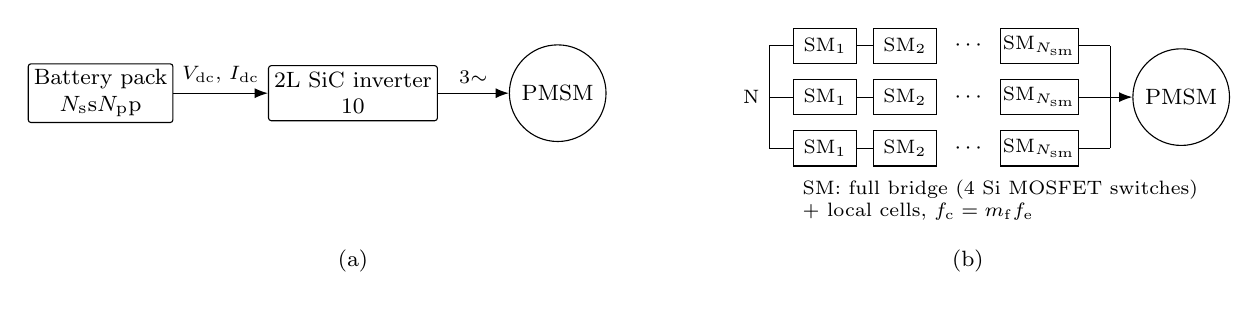
\begin{tikzpicture}[font=\footnotesize, >=Latex,
  blk/.style={draw, rounded corners=1pt, minimum height=7mm, align=center, inner sep=2pt},
  sm/.style={draw, minimum width=8mm, minimum height=4.5mm, inner sep=1pt, font=\scriptsize}]
  % (a) two-level
  \node[blk, minimum width=17mm] (pack) {Battery pack\\$N_\mathrm{s}$s$N_\mathrm{p}$p};
  \node[blk, right=12mm of pack, minimum width=17mm] (inv) {2L SiC inverter\\\SI{10}{\kilo\hertz}};
  \node[draw, circle, right=9mm of inv, minimum size=9mm] (m1) {PMSM};
  \draw[->] (pack) -- node[above, font=\scriptsize]{$V_\mathrm{dc}$, $I_\mathrm{dc}$} (inv);
  \draw[->] (inv) -- node[above, font=\scriptsize]{3$\sim$} (m1);
  \node[font=\footnotesize] at ($(inv.south)+(0,-17.75mm)$) {(a)};
  % (b) BI-MMC
  \begin{scope}[xshift=92mm, yshift=6mm]
    \foreach \ph/\y in {a/0, b/-6.5mm, c/-13mm} {
      \node[sm] (s1\ph) at (0,\y) {SM$_1$};
      \node[sm, right=2mm of s1\ph] (s2\ph) {SM$_2$};
      \node[right=1mm of s2\ph] (d\ph) {$\cdots$};
      \node[sm, right=1mm of d\ph] (sn\ph) {SM$_{N_\mathrm{sm}}$};
      \draw (s1\ph) -- (s2\ph);
      \draw (sn\ph.east) -- ++(4mm,0) coordinate (o\ph);
      \draw (s1\ph.west) -- ++(-3mm,0) coordinate (n\ph);
    }
    \draw (na) -- (nc);
    \node[left=0mm of nb, font=\scriptsize] {N};
    \node[draw, circle, minimum size=9mm] (m2) at ($(ob)+(9mm,0)$) {PMSM};
    \draw (oa) -- (ob) -- (oc);
    \draw[->] (ob) -- (m2);
    \node[font=\scriptsize, align=left, anchor=north west] at ($(s1c.south west)+(0,-0.5mm)$)
      {SM: full bridge (4 Si MOSFET switches)\\+ local cells, $f_\mathrm{c}=m_\mathrm{f}f_\mathrm{e}$};
    \node[font=\footnotesize] at ($(s2c.south)+(8mm,-12mm)$) {(b)};
  \end{scope}
\end{tikzpicture}
\caption{Compared architectures: (a) battery pack with a two-level SiC inverter; (b) BI-MMC with three star-connected strings of $\Nsm$ battery-integrated full-bridge submodules. Each SM holds $\Nssm$ series and $\Npsm$ parallel cells.}
\label{fig:topologies}
\end{figure}

\paragraph{Two-level drive.} The pack has $N_\mathrm{s}$ series and $N_\mathrm{p}$ parallel cells and feeds a three-phase, six-switch SiC inverter (Wolfspeed EDB005M12TM4 \cite{wolfspeed_edb005}, $N_\mathrm{p,mos}$ devices in parallel per switch). The inverter switches the pack voltage $V_\mathrm{dc}$ at the fixed carrier frequency $f_\mathrm{sw}$ (default \SI{10}{\kilo\hertz}). The pack carries only the DC current $I_\mathrm{dc}$, which is the active-power current plus the converter losses.

\paragraph{AC battery.} Each of the three phases is a string of $\Nsm$ full-bridge SMs. An SM contains $\Nssm$ series and $\Npsm$ parallel cells and four Si MOSFET switches (each $N_\mathrm{p,mos}$ devices in parallel; Infineon IQDH29NE2LM5CGSC data for the on-resistance). The SM output is $+v_\mathrm{s}$, $0$ or $-v_\mathrm{s}$. The phase voltage is the sum of the inserted SM voltages, so the phase-voltage amplitude is at most $\Nsm\Nssm V_\mathrm{cell}$. The carrier frequency is $f_\mathrm{c}=m_\mathrm{f}f_\mathrm{e}$, i.e.\ a \emph{multiple of the fundamental frequency} (pulse number $m_\mathrm{f}$, default 2), not a fixed value. Because the cells are in series with the load, the cell current equals the phase current whenever the SM is inserted.

\paragraph{What is held equal.} Both drives share the machine, the cell type (\SI{24}{\ampere\hour} NMC) and the installed energy $E_\mathrm{b}$ (up to the rounding of the cell counts). The BI-MMC is sized from the number of series cells per SM so that it reaches at least the phase voltage the 2L inverter reaches with space-vector modulation (\cref{sec:sizing}). The efficiency in this paper covers the \emph{converter and battery losses only}; machine losses (copper, iron, mechanical) are not included, for either drive (see \cref{sec:discussion}).

\paragraph{Notation.} \Cref{tab:notation} lists the main symbols and the corresponding names in the code. All dq quantities are \emph{peak} (amplitude-invariant) values. Phase quantities of the machine are rotor-synchronous: $\omega_\mathrm{e}=p\,\omega_\mathrm{m}$ with $\omega_\mathrm{m}$ the mechanical speed in \si{\radian\per\second}.

\begin{table}[ht]
\centering
\caption{Main symbols and their names in the Python code.}
\label{tab:notation}
\footnotesize
\setlength\tabcolsep{4pt}
\begin{tabular}{@{}llll@{}}
\toprule
Symbol & Meaning & Unit & Code \\
\midrule
$P_\mathrm{b}$, $\omega_\mathrm{b}$, $T_\mathrm{b}$ & base power, speed, torque & W, rad/s, N\,m & \code{PBase}, \code{wmBase}, \code{TBase} \\
$V_\mathrm{b}$, $V_\mathrm{max}$ & base and maximum phase voltage (peak) & V & \code{VBase}, \code{VMax} \\
$I_\mathrm{b}$ & peak current limit & A & \code{Ibase} \\
$\psi_\mathrm{f}$, $R_\mathrm{s}$, $L_\mathrm{d}$, $L_\mathrm{q}$ & machine parameters & Wb, \si{\ohm}, H & \code{magnet_flux}, \dots \\
$i_\mathrm{d}$, $i_\mathrm{q}$, $v_\mathrm{d}$, $v_\mathrm{q}$ & dq currents and voltages (peak) & A, V & \code{Id}, \code{Iq}, \code{Vd}, \code{Vq} \\
$\Ihat$ & stator current amplitude $\sqrt{i_\mathrm{d}^2+i_\mathrm{q}^2}$ & A & \\
$T$, $P_\mathrm{out}$ & shaft torque, shaft power $\omega_\mathrm{m}T$ & N\,m, W & \code{T}, \code{Pout} \\
$z$ & cell state of charge & -- & \code{soc} \\
$V_\mathrm{cell}$, $R_0$, $R_1$, $C_1$ & cell OCV and equivalent circuit & V, \si{\ohm}, \si{\ohm}, F & \code{cell_state()} \\
$N_\mathrm{s}$, $N_\mathrm{p}$ & series and parallel cells of the 2L pack & -- & \code{Nscells_2l}, \code{Npcells_2l} \\
$\Nsm$, $\Nssm$, $\Npsm$ & SMs per phase, series and parallel cells per SM & -- & \code{Nsm}, \code{Nscells_b}, \code{Npcells_b} \\
$r$ & redundant SM share & pu & \code{Nsm_redundant_pu} \\
$N_\mathrm{p,mos}$ & parallel devices per switch & -- & \code{Npmos_2l}, \code{Npmos_b} \\
$\Rds$ & on-resistance & \si{\ohm} & \code{Rdson_2l}, \code{Rdson_bimmc} \\
$f_\mathrm{sw}$, $m_\mathrm{f}$ & 2L carrier frequency, BI-MMC pulse number & Hz, -- & \code{fsw}, \code{mf_bimmc} \\
$P_\mathrm{c}$, $P_\mathrm{s}$, $P_\mathrm{b}$ & conduction, switching, battery loss & W & \code{Pc}, \code{Ps}, \code{Pb} \\
$\Tj$, $\Tc$, $T_\mathrm{cell}$ & junction, case, cell temperature & \si{\celsius} & \code{Tj}, \code{Tc}, \code{Tcell} \\
\bottomrule
\end{tabular}
\end{table}

\section{Software Architecture}\label{sec:software}
The platform is a Python package in the folder \code{python/} of the repository. It has no build step; the dependencies are NumPy, SciPy, pandas, matplotlib, CasADi \cite{andersson2019} with IPOPT \cite{waechter2006}, Numba \cite{lam2015}, tqdm, openpyxl and, for the dashboard, Streamlit. \Cref{tab:modules} lists the modules, and \cref{fig:flow} shows how the two analyses use them.

\begin{table}[ht]
\centering
\caption{Modules of the Python package (\code{python/}).}
\label{tab:modules}
\footnotesize
\setlength\tabcolsep{4pt}
\begin{tabular}{@{}p{3.2cm}p{13.3cm}@{}}
\toprule
Module & Role \\
\midrule
\code{calc.py} & Low-level physics: MTPA optimisation problem (CasADi/IPOPT), 2L and BI-MMC loss functions, equivalent-circuit battery simulation (Numba-compiled). Dataclasses for the machine, switching slopes, battery, thermal network and converter configuration. \\
\code{model.py} & Headless model shared by all front ends: user-input dictionary \code{NOMINAL}, derived design (\code{design}), cell state (\code{cell_state}), MOSFET data and Rdson(Tj) fits, MTPA over a grid (\code{solve_mtpa}), dq voltages, \code{loss_maps}, \code{efficiency}. \\
\code{applications.py} & Presets of the six applications (drive rating, vehicle data, duty cycle), the road-load force and the gear ratio. \\
\code{cycles.py} & Conversion of a duty cycle to a machine speed and torque time series (five cycle kinds). \\
\code{cycle_eval.py} & Analysis~II: sample-by-sample cycle loss evaluation with SOC and temperature tracking, summary metrics, command-line driver. \\
\code{create_maps_PCIM.py} & Analysis~I for every application: MTPA, loss, temperature and efficiency maps as figures (and Excel data). \\
\code{main.py} & Streamlit dashboard for Analysis~I with interactive inputs. \\
\code{plots.py}, \code{export.py} & Map figures (matplotlib) and Excel export of all plotted data. \\
\code{sens.py} & One-at-a-time sensitivity of both efficiencies at one operating point. \\
\code{fit_rdson.py} & Polynomial fit of normalised Rdson versus Tj from datasheet points. \\
\code{test.py} & Interactive script that evaluates and plots one cycle. \\
\code{data/} & Datasheet curves (CSV) and the public duty cycles (\code{data/cycles/}, with a README on provenance). \\
\bottomrule
\end{tabular}
\end{table}

\begin{figure}[ht]
\centering
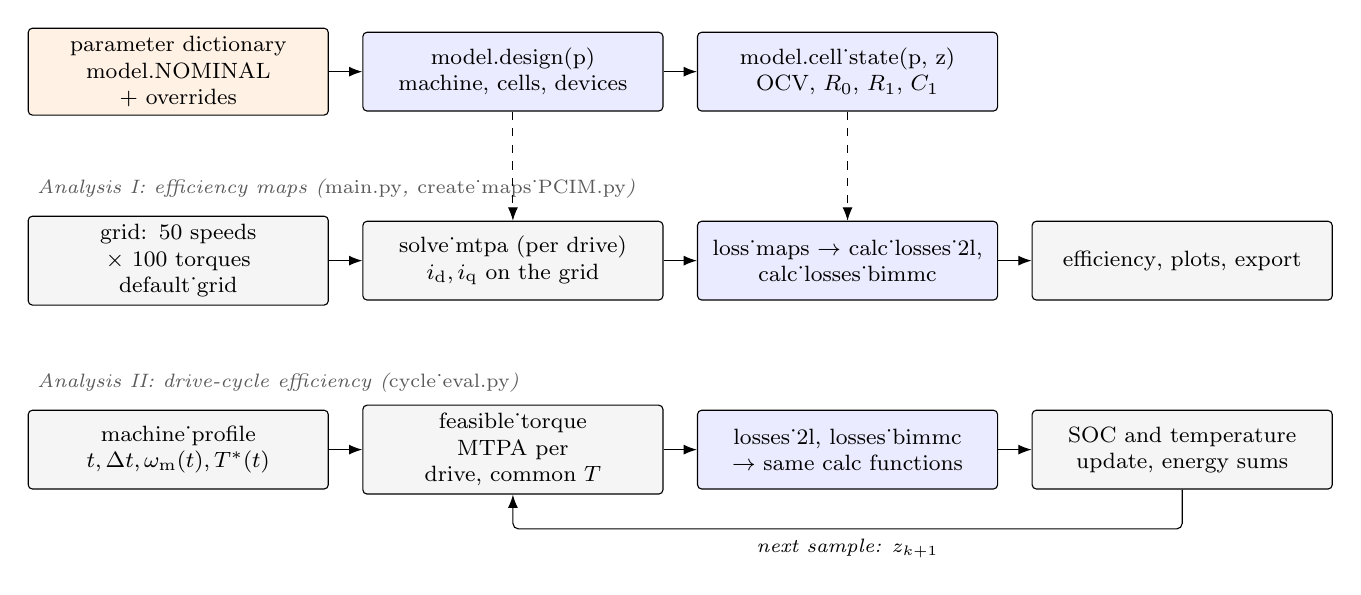
\begin{tikzpicture}[font=\footnotesize, >=Latex,
  box/.style={draw, rounded corners=1.5pt, align=center, inner sep=3pt, minimum height=10mm, minimum width=38mm, text width=36mm, fill=black!4},
  core/.style={box, fill=blue!8},
  io/.style={box, fill=orange!10},
  lab/.style={font=\scriptsize\itshape, text=black!65, anchor=south west}]
  \def\dx{42.5mm}\def\dy{-24mm}
  % inputs
  \node[io] (p) at (0,0) {parameter dictionary\\ \code{model.NOMINAL} + overrides};
  \node[core] (des) at (\dx,0) {\code{model.design(p)}\\ machine, cells, devices};
  \node[core] (cell) at (2*\dx,0) {\code{model.cell_state(p, z)}\\ OCV, $R_0$, $R_1$, $C_1$};
  \draw[->] (p) -- (des); \draw[->] (des) -- (cell);
  % Analysis I
  \node[box] (grid) at (0,\dy) {grid: 50 speeds $\times$ 100 torques\\ \code{default_grid}};
  \node[box] (mtpa) at (\dx,\dy) {\code{solve_mtpa} (per drive)\\ $i_\mathrm{d}, i_\mathrm{q}$ on the grid};
  \node[core] (lm) at (2*\dx,\dy) {\code{loss_maps} $\to$ \code{calc_losses_2l}, \code{calc_losses_bimmc}};
  \node[box] (eff) at (3*\dx,\dy) {\code{efficiency}, \code{plots}, \code{export}};
  \draw[->] (grid) -- (mtpa); \draw[->] (mtpa) -- (lm); \draw[->] (lm) -- (eff);
  \node[lab] at ($(grid.north west)+(0,1mm)$) {Analysis I: efficiency maps (\code{main.py}, \code{create_maps_PCIM.py})};
  % Analysis II
  \node[box] (cyc) at (0,2*\dy) {\code{machine_profile}\\ $t,\Delta t,\omega_\mathrm{m}(t),T^*(t)$};
  \node[box] (feas) at (\dx,2*\dy) {\code{feasible_torque}\\ MTPA per drive, common $T$};
  \node[core] (lc) at (2*\dx,2*\dy) {\code{losses_2l}, \code{losses_bimmc} $\to$ same \code{calc} functions};
  \node[box] (soc) at (3*\dx,2*\dy) {SOC and temperature update, energy sums};
  \draw[->] (cyc) -- (feas); \draw[->] (feas) -- (lc); \draw[->] (lc) -- (soc);
  \draw[->, rounded corners=2pt] (soc.south) -- ++(0,-5mm) -| node[font=\scriptsize\itshape, pos=0.25, below]{next sample: $z_{k+1}$} (feas.south);
  \node[lab] at ($(cyc.north west)+(0,1mm)$) {Analysis II: drive-cycle efficiency (\code{cycle_eval.py})};
  % shared inputs
  \draw[->, dashed] (des.south) -- (mtpa.north);
  \draw[->, dashed] (cell.south) -- (lm.north);
\end{tikzpicture}
\caption{Data flow of the two analyses. Both read the same parameter dictionary, the same derived design and the same cell model, and both end in the same two loss functions of \code{calc.py}. They differ only in how the operating points are generated (a fixed grid versus a duty cycle) and in what is accumulated. Dashed: shared inputs of Analysis~I; Analysis~II calls \code{cell_state} and the MTPA solver at every sample with the present SOC.}
\label{fig:flow}
\end{figure}

\paragraph{Parameter dictionary.} All user inputs are collected in one dictionary in the format of \code{model.NOMINAL} (\cref{tab:params} in the appendix). The dashboard fills it from the sidebar, \code{applications.py} overrides a few entries per application, and \code{sens.py} sweeps entries one at a time. No module keeps hidden state, so a result is a pure function of this dictionary, the SOC and the grid or cycle.

\paragraph{Two parameter sets.} The dashboard and \code{create_maps_PCIM.py} default to the settings of the original dashboard: both drives are limited to the 2L voltage and the on-resistance is constant. The cycle evaluation and this paper use the improved settings of \code{model.py}: each drive has its own voltage limit, and $\Rds$ follows the junction temperature. These are the switches \code{voltage_limit} and \code{rdson_tj} of \code{model.loss_maps}. All maps in this paper use the improved settings, so both analyses use the same model. The BI-MMC sizing (\cref{eq:npsm}) is identical in all front ends.

\paragraph{Running the analyses.}
\begin{lstlisting}[numbers=none, language={}]
streamlit run main.py                                   # dashboard (maps)
python create_maps_PCIM.py --apps car bus --soc 0.5     # maps per application
python cycle_eval.py --apps car bus --soc 0.2 0.5 0.9   # drive cycles
python sens.py --speed-pu 1.0 --torque-pu 0.8           # sensitivity
python fit_rdson.py --degree 3 --plot                   # Rdson fit
\end{lstlisting}
Cycle jobs (application $\times$ initial SOC) run in parallel with a process pool; the 18 jobs of this paper take about \SI{20}{\second} on a laptop. Map computation takes about ten seconds per application, dominated by the time-domain battery simulation of the BI-MMC.

\paragraph{Outputs.} Analysis~II writes \code{cycle_results.json/xlsx} (one row per application and SOC) and one trace CSV per job. Analysis~I writes PNG figures and, optionally, one Excel workbook with the data behind every plot (speed--torque maps as torque $\times$ speed blocks). \Cref{app:outputs} lists the formats. A static browser port of the dashboard is in \code{pages/}; this paper documents the Python implementation only.

\section{Models Shared by Both Analyses}\label{sec:models}
This section gives every equation used by the code. The MTPA problem and the two loss functions are identical in both analyses.

\subsection{Machine and base values}\label{sec:design}
The machine is specified by its base power $P_\mathrm{b}$, base speed $n_\mathrm{b}$ (rpm), DC voltage $V_\mathrm{dc}$, pole pairs $p$ and the per-unit parameters $r_\mathrm{s}$, $l_\mathrm{d}$, $l_\mathrm{q}$. \code{model.design} derives
\begin{align}
V_\mathrm{b}&=\tfrac12 V_\mathrm{dc}, & V_\mathrm{max}&=\tfrac{2}{\sqrt3}V_\mathrm{b}=\tfrac{V_\mathrm{dc}}{\sqrt3}, & \omega_\mathrm{b}&=\tfrac{2\pi}{60}n_\mathrm{b}, & T_\mathrm{b}&=\tfrac{P_\mathrm{b}}{\omega_\mathrm{b}}, \label{eq:base1}\\
\psi_\mathrm{f}&=\frac{V_\mathrm{b}}{\omega_\mathrm{b}\,p}, & Z_\mathrm{b}&=\frac{\big(\sqrt{3/2}\,V_\mathrm{b}\big)^2}{P_\mathrm{b}}, & I_\mathrm{b}&=50\left\lceil\frac{1}{50}\,\frac{2P_\mathrm{b}}{3V_\mathrm{b}}\right\rceil, \label{eq:base2}\\
R_\mathrm{s}&=r_\mathrm{s}Z_\mathrm{b}, & L_\mathrm{d}&=\frac{l_\mathrm{d}Z_\mathrm{b}}{\omega_\mathrm{b}p}, & L_\mathrm{q}&=\frac{l_\mathrm{q}Z_\mathrm{b}}{\omega_\mathrm{b}p}, \label{eq:base3}\\
\omega_\mathrm{m,max}&=\frac{V_\mathrm{max}}{p\,(\psi_\mathrm{f}-L_\mathrm{d}I_\mathrm{b})}. \label{eq:wmax}
\end{align}
$V_\mathrm{b}$ is a peak phase voltage and $I_\mathrm{b}$ a peak current (rounded up to a multiple of \SI{50}{\ampere}). The magnet flux is chosen so that the back-EMF at base speed equals $V_\mathrm{b}$, and $Z_\mathrm{b}$ is the line-to-line base impedance, which equals $V_\mathrm{b}/I_\mathrm{b}$ before rounding. \Cref{eq:wmax} is the speed at which the voltage limit is reached with the full current $I_\mathrm{b}$ in the negative d axis, neglecting $R_\mathrm{s}$ and $L_\mathrm{q}$; it sets the upper end of the speed range. The code raises an error if $L_\mathrm{d}I_\mathrm{b}\ge\psi_\mathrm{f}$ (no finite maximum speed). \Cref{tab:machine} lists the derived values of the six applications.

\begin{table}[ht]
\centering
\caption{Machine rating and derived machine data of the six applications ($p=4$, $r_\mathrm{s}=0.01$, $l_\mathrm{d}=0.55$, $l_\mathrm{q}=0.85$ pu for all).}
\label{tab:machine}
\footnotesize
\begin{tabular}{@{}lrrrrrrrrrrr@{}}
\toprule
Application & $P_\mathrm{b}$ & $n_\mathrm{b}$ & $V_\mathrm{dc}$ & $E_\mathrm{b}$ & $T_\mathrm{b}$ & $I_\mathrm{b}$ & $n_\mathrm{max}$ & $\psi_\mathrm{f}$ & $R_\mathrm{s}$ & $L_\mathrm{d}$ & $L_\mathrm{q}$ \\
 & [kW] & [rpm] & [V] & [kWh] & [N\,m] & [A] & [rpm] & [mWb] & [m\si{\ohm}] & [\si{\micro\henry}] & [\si{\micro\henry}] \\
\midrule
Passenger car & 150 & 5000 & 400 & 75 & 286 & 500 & 12830 & 95.5 & 4.00 & 105 & 162 \\
City bus & 350 & 2500 & 700 & 350 & 1337 & 700 & 6833 & 334.2 & 5.25 & 276 & 426 \\
Heavy-duty truck & 550 & 3000 & 700 & 400 & 1751 & 1050 & 7719 & 278.5 & 3.34 & 146 & 226 \\
Off-road machine & 150 & 2000 & 700 & 200 & 716 & 300 & 5466 & 417.8 & 12.25 & 804 & 1243 \\
Marine vessel & 400 & 1800 & 800 & 1000 & 2122 & 700 & 4919 & 530.5 & 6.00 & 438 & 676 \\
Regional train & 600 & 2000 & 800 & 300 & 2865 & 1000 & 5132 & 477.5 & 4.00 & 263 & 406
\\
\bottomrule
\end{tabular}
\end{table}

\subsection{Cell model and battery sizing}\label{sec:sizing}
\paragraph{Cell.} The cell is described by its open-circuit voltage (OCV) $V_\mathrm{cell}(z)$, a table in the SOC $z$ (\cref{tab:ocv} in the appendix; linear interpolation), and a first-order equivalent circuit (series $R_0$, parallel $R_1\parallel C_1$). The parameters follow from nominal values and second-order scaling polynomials in $z$ (\code{model.cell_state}):
\begin{equation}
R_0(z)=R_{0,\mathrm{nom}}\,\pi_\mathrm{r}(z),\quad R_1(z)=R_{1,\mathrm{nom}}\,\pi_\mathrm{r}(z),\quad C_1(z)=C_{1,\mathrm{nom}}\,\pi_\mathrm{c}(z),
\label{eq:cellrc}
\end{equation}
with $\pi_\mathrm{r}(z)=1.3z^2-1.3z+1.3$, $\pi_\mathrm{c}(z)=-1.3z^2+1.3z+1.3$ (defaults for the Samsung PHEV2 \SI{24}{\ampere\hour} cell), $R_{0,\mathrm{nom}}=\SI{1.2}{\milli\ohm}$, $R_{1,\mathrm{nom}}=\SI{0.7}{\milli\ohm}$, and $C_{1,\mathrm{nom}}=1/(2\pi\cdot\SI{250}{\hertz}\cdot R_{1,\mathrm{nom}})$ so that the RC corner is \SI{250}{\hertz}. \Cref{fig:cell} shows the OCV and the parameters.

\begin{figure}[ht]
\centering
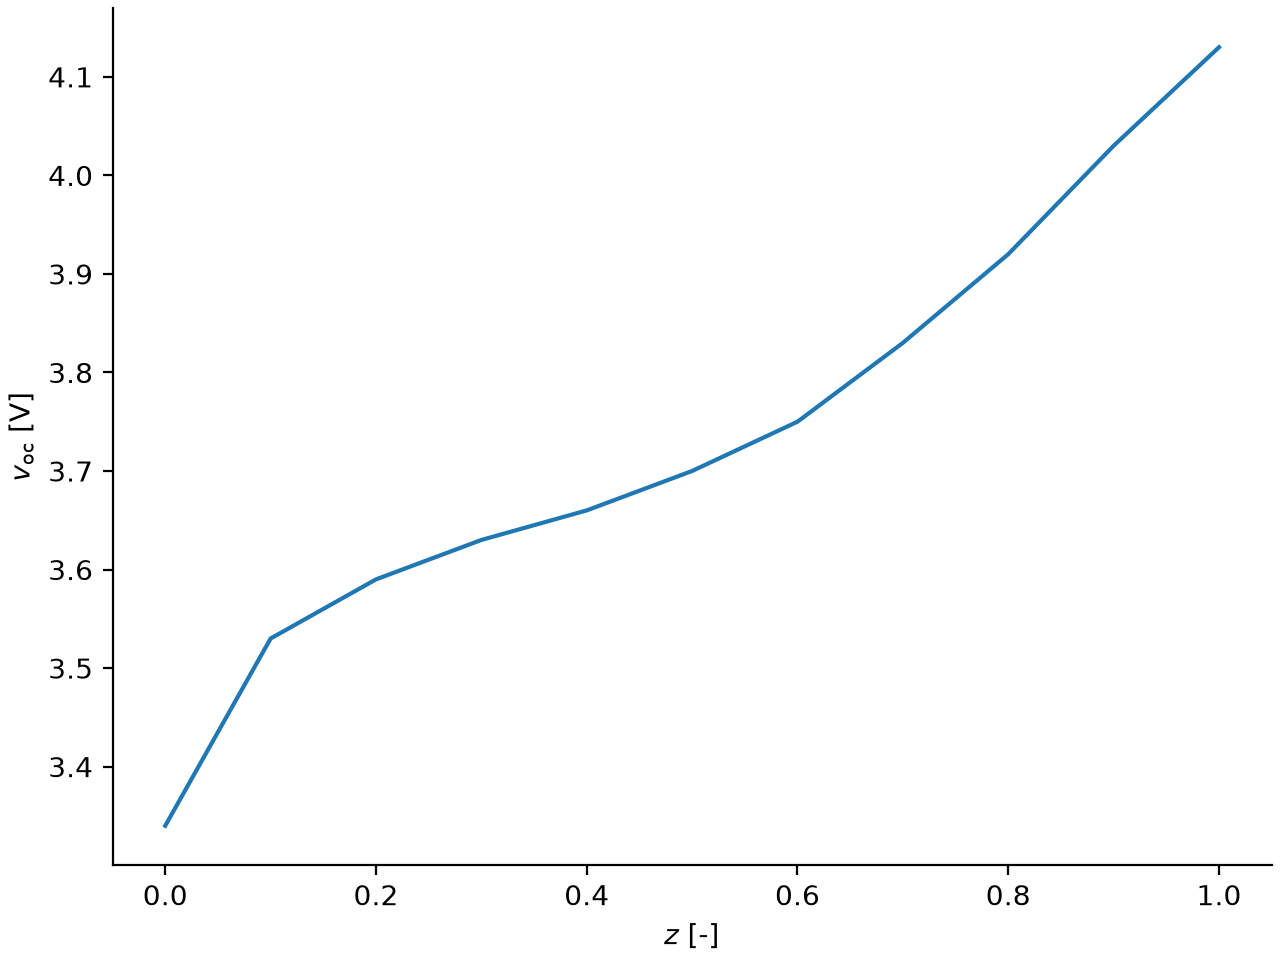
\includegraphics[width=0.48\linewidth]{figures/inputs/battery_ocv.png}\hfill
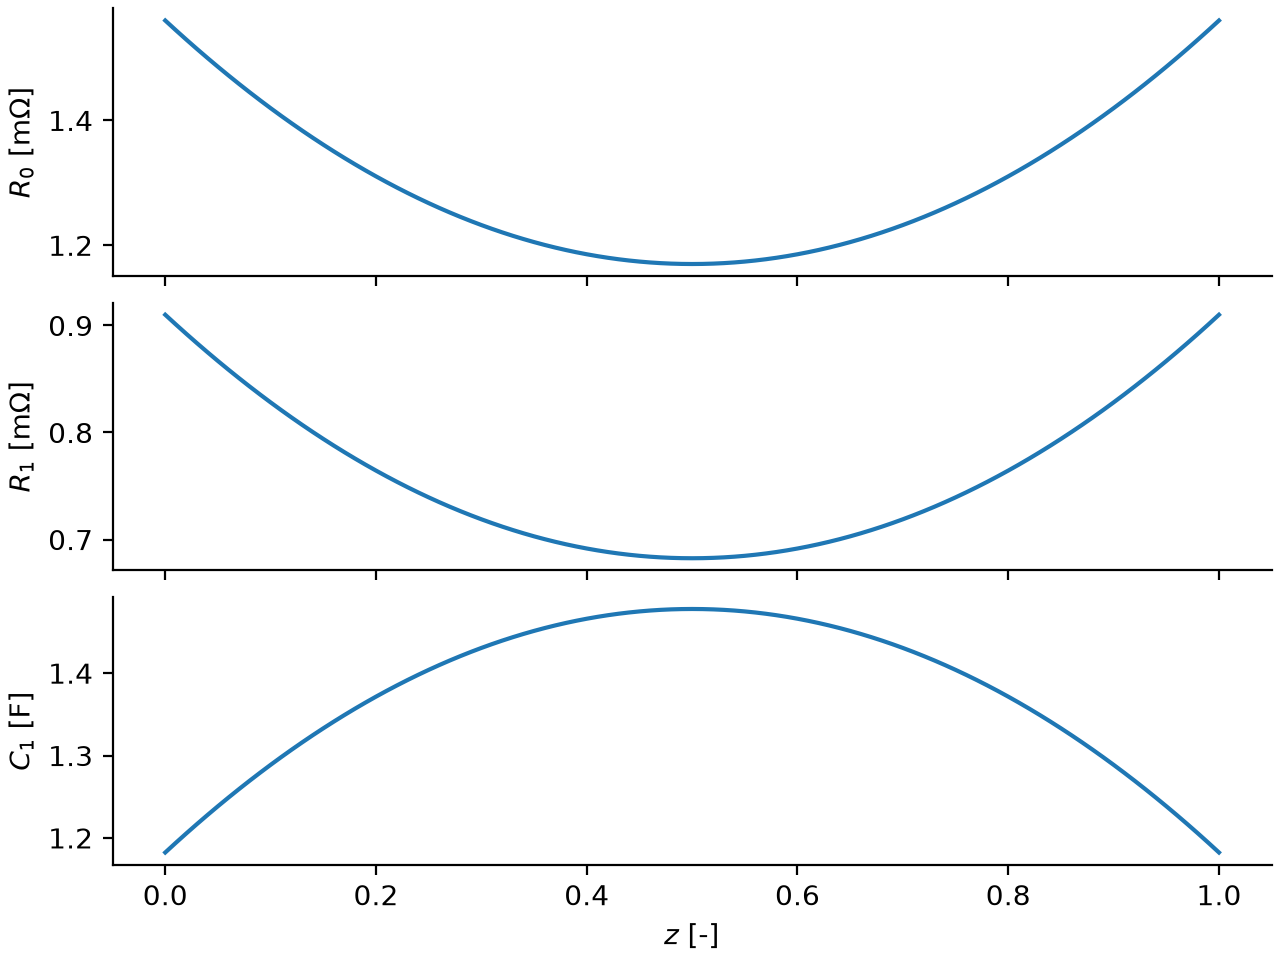
\includegraphics[width=0.48\linewidth]{figures/inputs/battery_parameters.png}
\caption{Cell data of the NMC cell: open-circuit voltage versus SOC (left) and the SOC-scaled equivalent-circuit parameters (right).}
\label{fig:cell}
\end{figure}

\paragraph{Thermal model of the cell.} Cells are cooled from the bottom, insulated on the sides, with the coolant at the ambient temperature. The steady-state cell temperature for a battery loss $P_\mathrm{b}$ shared equally by $n$ cells is
\begin{equation}
T_\mathrm{cell}=T_\mathrm{amb}+\frac{P_\mathrm{b}}{n}R_\mathrm{th,cell},\qquad R_\mathrm{th,cell}=\frac{l_\mathrm{z}}{k_\mathrm{z}A_\mathrm{z}}=\frac{\SI{0.027}{\metre}}{\SI{25}{\watt\per\metre\per\kelvin}\cdot\SI{3.996e-3}{\metre\squared}}=\SI{0.27}{\kelvin\per\watt}.
\label{eq:tcell}
\end{equation}

\paragraph{2L pack.} With $V_\mathrm{nom}=V_\mathrm{cell}(0.5)$,
\begin{equation}
N_\mathrm{s}=\Big\lceil\frac{V_\mathrm{dc}}{V_\mathrm{nom}}\Big\rceil,\qquad N_\mathrm{p}=\Big\lceil\frac{E_\mathrm{b}}{Q_\mathrm{cell}V_\mathrm{nom}N_\mathrm{s}}\Big\rceil.
\label{eq:pack2l}
\end{equation}
The DC-link voltage at the present SOC is $V_\mathrm{dc}(z)=N_\mathrm{s}V_\mathrm{cell}(z)$.

\paragraph{BI-MMC sizing.} The user chooses the number of series cells per submodule, $\Nssm$ (default 10); the number of submodules and parallel cells follow. The BI-MMC phase-voltage amplitude is $\Nsm\Nssm V_\mathrm{cell}(1-r)$, where $r$ is the redundant share of the $\Nsm$ SMs, and it must reach the peak phase voltage $V_\mathrm{max}$ of \cref{eq:base1} at the nominal cell voltage. Rounding up (\code{model.design}),
\begin{equation}
\Nsm=\Big\lceil\frac{V_\mathrm{max}}{V_\mathrm{nom}\,\Nssm\,(1-r)}\Big\rceil,\qquad
\Npsm=\Big\lceil\frac{E_\mathrm{b}}{3\,\Nsm\,\Nssm\,V_\mathrm{nom}\,Q_\mathrm{cell}}\Big\rceil.
\label{eq:npsm}
\end{equation}
The 2L inverter with space-vector modulation reaches $V_\mathrm{dc}/\sqrt3=V_\mathrm{max}$ at the same cell voltage. Because $\Nsm$ and $\Npsm$ are integers, the BI-MMC string voltage is \SIrange{0.7}{4.1}{\percent} above $V_\mathrm{max}$ and the BI-MMC has between $-0.8$ and $+8.4$~\% more cells than the 2L pack (\cref{tab:conv}). Choosing $\Nssm$ per application keeps these deviations small; the passenger car uses $\Nssm=7$ instead of the default, because 10 series cells would give 7 SMs and \SI{20}{\percent} more cells than the 2L pack.

\paragraph{Parallel devices.} The 2L switch needs $N_\mathrm{p,mos}=\lceil I_\mathrm{b}/(\sqrt2 I_\mathrm{rated})\rceil$ devices ($I_\mathrm{rated}=\SI{320}{\ampere}$ RMS). The BI-MMC switch uses $\max\big(\lceil I_\mathrm{b}/(\sqrt2\cdot\SI{400}{\ampere})\rceil,\,4\big)$ devices. \Cref{tab:conv} lists the resulting design of every application.

\begin{table}[ht]
\centering
\caption{Battery and converter design of the six applications (\cref{eq:pack2l,eq:npsm}; cell energy as in \cref{tab:machine}). $N_\mathrm{cells}$ is the total cell count of each drive.}
\label{tab:conv}
\footnotesize
\begin{tabular}{@{}lccccrrr@{}}
\toprule
Application & 2L pack & $N_\mathrm{p,mos}$ (2L) & $\Nsm\times\Nssm$ & $\Npsm$ & $N_\mathrm{p,mos}$ (BI) & $N_\mathrm{cells}$ (2L) & $N_\mathrm{cells}$ (BI) \\
\midrule
Passenger car & $109\mathrm{s}8\mathrm{p}$ & 2 & $9\times7$ & 5.00 & 4 & 872 & 945 \\
City bus & $190\mathrm{s}21\mathrm{p}$ & 2 & $11\times10$ & 12.00 & 4 & 3990 & 3960 \\
Heavy-duty truck & $190\mathrm{s}24\mathrm{p}$ & 3 & $11\times10$ & 14.00 & 4 & 4560 & 4620 \\
Off-road machine & $190\mathrm{s}12\mathrm{p}$ & 1 & $11\times10$ & 7.00 & 4 & 2280 & 2310 \\
Marine vessel & $217\mathrm{s}52\mathrm{p}$ & 2 & $13\times10$ & 29.00 & 4 & 11284 & 11310 \\
Regional train & $217\mathrm{s}16\mathrm{p}$ & 3 & $13\times10$ & 9.00 & 4 & 3472 & 3510
\\
\bottomrule
\end{tabular}
\end{table}

\subsection{MTPA control}\label{sec:mtpa}
In the rotor frame, the stator voltage equations (steady state) and the torque of the PMSM are
\begin{align}
v_\mathrm{d}&=R_\mathrm{s}i_\mathrm{d}-\omega_\mathrm{e}L_\mathrm{q}i_\mathrm{q}, \label{eq:vd}\\
v_\mathrm{q}&=R_\mathrm{s}i_\mathrm{q}+\omega_\mathrm{e}\big(\psi_\mathrm{f}+L_\mathrm{d}i_\mathrm{d}\big), \label{eq:vq}\\
T&=\tfrac32 p\big(\psi_\mathrm{f}i_\mathrm{q}+(L_\mathrm{d}-L_\mathrm{q})i_\mathrm{d}i_\mathrm{q}\big), \label{eq:torque}
\end{align}
with $\omega_\mathrm{e}=p\,\omega_\mathrm{m}$ (\code{model.dq_voltages}). For every operating point $(\omega_\mathrm{m},T^*)$ the code solves the optimisation problem (\code{calc.create_mtpa_optimization_problem})
\begin{equation}
\min_{i_\mathrm{d},i_\mathrm{q}}\; i_\mathrm{d}^2+i_\mathrm{q}^2\quad\text{s.t.}\quad T(i_\mathrm{d},i_\mathrm{q})=T^*,\qquad v_\mathrm{d}^2+v_\mathrm{q}^2< \hat v_\mathrm{max}^2,
\label{eq:mtpa}
\end{equation}
that is, the minimum-current solution that produces the requested torque and respects the voltage limit. It is therefore MTPA below base speed and automatically adds field weakening (negative $i_\mathrm{d}$) when the voltage limit becomes active. The problem is built once with CasADi's \code{Opti} stack, with $T^*$, $\omega_\mathrm{m}$ and $\hat v_\mathrm{max}$ as parameters, and solved with IPOPT (print level 0). Because the torque constraint is bilinear, the problem is non-convex; the previous solution warm-starts the next solve, which in practice keeps the solver on the MTPA branch. After the solve, two checks are applied. A point is marked infeasible (NaN) if IPOPT fails (voltage limit cannot be met), if its power exceeds the rating ($|\omega_\mathrm{m}T^*|>P_\mathrm{b}$, skipped before solving), or if the current exceeds the limit, $i_\mathrm{d}^2+i_\mathrm{q}^2>I_\mathrm{b}^2$. After a failure, the initial guess is reset to zero.

\paragraph{Voltage limit per drive.} The limit $\hat v_\mathrm{max}$ follows the cell OCV at the present SOC and differs between the drives:
\begin{equation}
\hat v_\mathrm{max}^\mathrm{2L}=\frac{N_\mathrm{s}V_\mathrm{cell}(z)}{\sqrt3},\qquad
\hat v_\mathrm{max}^\mathrm{BI}=\Nssm V_\mathrm{cell}(z)\,\Nsm\,(1-r).
\label{eq:vmax}
\end{equation}
The factor $(1-r)$ accounts for the redundant SM share $r$ (default $r=0$). By construction of \cref{eq:npsm}, the BI-MMC limit is equal to or slightly above the 2L limit (by the rounding of $\Nsm$). If both limits are equal, the code solves the MTPA problem once and reuses the currents for both drives.

\subsection{Two-level inverter losses}\label{sec:loss2l}
\code{calc.calc_losses_2l} receives the dq currents and voltages and returns the conduction loss $P_\mathrm{c}$, the switching loss $P_\mathrm{s}$, the battery loss $P_\mathrm{b}$ and the temperatures $\Tj$, $\Tc$.

\paragraph{Conduction loss.} With the stator current amplitude $\Ihat=\sqrt{i_\mathrm{d}^2+i_\mathrm{q}^2}$ and a sinusoidal phase current, each switch conducts half the fundamental period. The RMS current of one device is $\Ihat/(\sqrt2N_\mathrm{p,mos})$, so a device dissipates $\tfrac12\big(\Ihat/(\sqrt2N_\mathrm{p,mos})\big)^2\Rds$ on average, a switch of $N_\mathrm{p,mos}$ devices $\tfrac14\Ihat^2\Rds/N_\mathrm{p,mos}$, and the six switches
\begin{equation}
P_\mathrm{c}^\mathrm{2L}=\frac32\,\Rds\,\frac{i_\mathrm{d}^2+i_\mathrm{q}^2}{N_\mathrm{p,mos}}.
\label{eq:pc2l}
\end{equation}
The model does not distinguish between the transistor and the body diode and ignores the dependence on the modulation index.

\paragraph{Switching loss.} The datasheet gives current- and voltage-slope curves $\mathrm{d}i/\mathrm{d}t$ and $\mathrm{d}v/\mathrm{d}t$ for turn-on and turn-off as functions of the device current (\cref{fig:slopes}); the code interpolates them linearly and holds them constant outside the data range. The average absolute phase current is $\bar\imath=\tfrac{2}{\pi}\Ihat$, the device current $\bar\imath_\mathrm{dev}=\bar\imath/N_\mathrm{p,mos}$, and the four commutation intervals follow from the slopes (slopes in units of per nanosecond):
\begin{equation}
t_\mathrm{ri}=\frac{\bar\imath_\mathrm{dev}}{(\mathrm{d}i/\mathrm{d}t)_\mathrm{on}},\quad
t_\mathrm{fi}=\frac{\bar\imath_\mathrm{dev}}{(\mathrm{d}i/\mathrm{d}t)_\mathrm{off}},\quad
t_\mathrm{rv}=\frac{V_\mathrm{dc}}{(\mathrm{d}v/\mathrm{d}t)_\mathrm{on}},\quad
t_\mathrm{fv}=\frac{V_\mathrm{dc}}{(\mathrm{d}v/\mathrm{d}t)_\mathrm{off}},
\label{eq:times}
\end{equation}
where the slopes are in \si{\ampere\per\nano\second} and \si{\volt\per\nano\second}, so the times are multiplied by $10^{-9}$ to obtain seconds. The slope-based energy per switching event of one switch follows the linear-overlap approach of \cite{graovac2006},
\begin{equation}
E_\mathrm{sw}=\tfrac12V_\mathrm{dc}\,\bar\imath\,\big(t_\mathrm{ri}+t_\mathrm{fv}+t_\mathrm{fi}+t_\mathrm{rv}\big),\qquad
P_\mathrm{s}^\mathrm{2L}=6\,E_\mathrm{sw}f_\mathrm{sw}.
\label{eq:ps2l}
\end{equation}
$E_\mathrm{sw}$ already covers all $N_\mathrm{p,mos}$ devices of one switch, because the device times scale with $\bar\imath_\mathrm{dev}$ and the energy of $N_\mathrm{p,mos}$ devices adds up. The factor 6 counts one switching event per switch and carrier period.

\begin{figure}[ht]
\centering
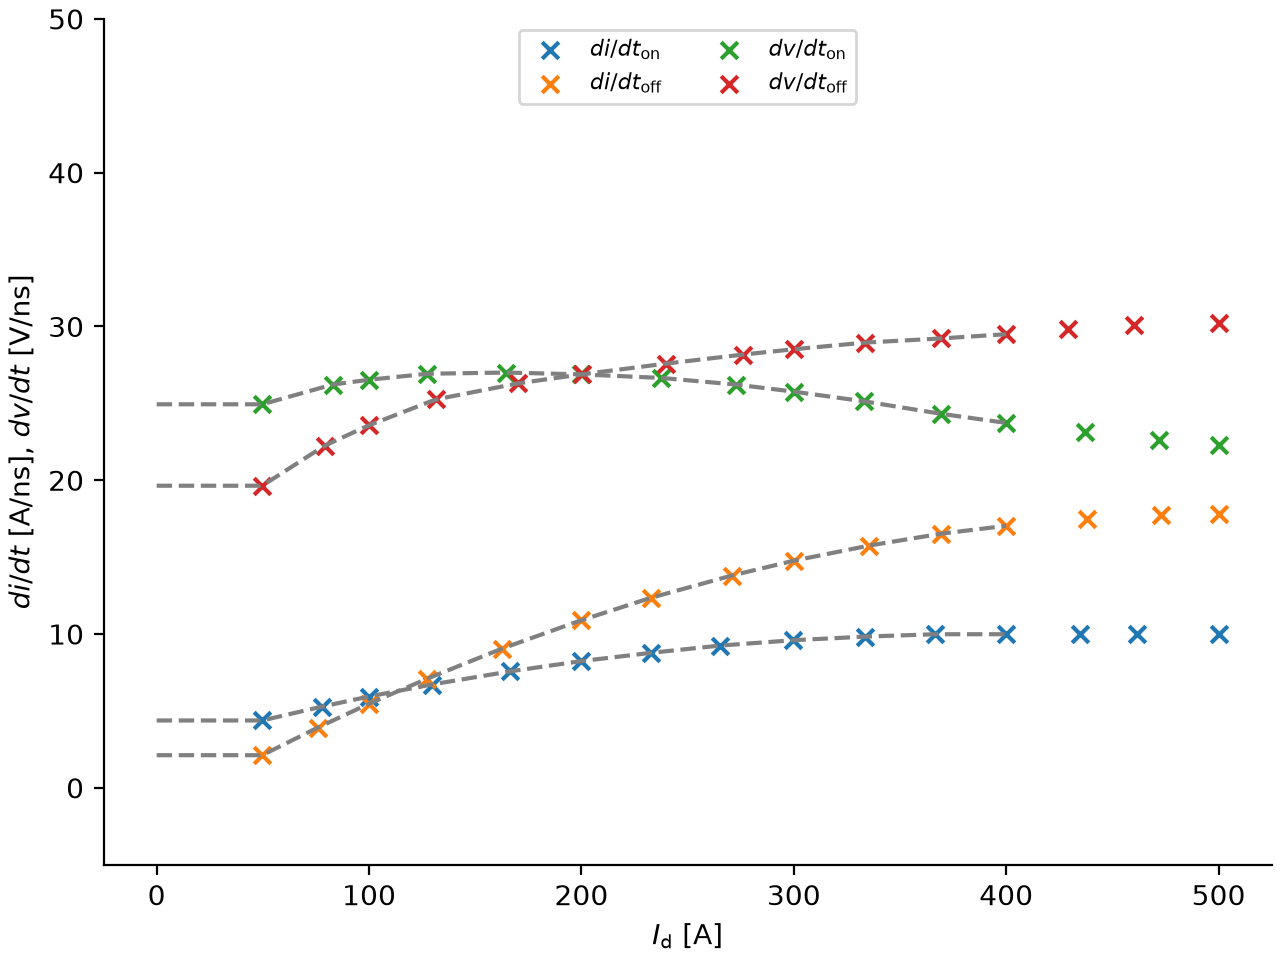
\includegraphics[width=0.62\linewidth]{figures/inputs/switching_slopes.png}
\caption{Switching slopes of the Wolfspeed EDB005M12TM4 as a function of the device current: datasheet points (crosses) and the linear interpolation used by the code (dashed).}
\label{fig:slopes}
\end{figure}

\paragraph{Temperatures and $\Rds(\Tj)$.} The loss per device, $P_\mathrm{dev}=(P_\mathrm{c}+P_\mathrm{s})/(6N_\mathrm{p,mos})$, flows through the case-to-ambient and junction-to-case thermal resistances in series (steady state):
\begin{equation}
\Tc=T_\mathrm{amb}+P_\mathrm{dev}R_\mathrm{th,ca},\qquad \Tj=\Tc+P_\mathrm{dev}R_\mathrm{th,jc}.
\label{eq:thermal2l}
\end{equation}
The on-resistance depends on $\Tj$. The datasheet curve, normalised to \SI{25}{\celsius}, is fitted by a cubic polynomial $\rho(\Tj)=c_3\Tj^3+c_2\Tj^2+c_1\Tj+c_0$ with $\rho(25)=1$ after normalisation (\code{model.rdson_poly_fun}, \code{fit_rdson.py}; \cref{fig:rdson}), and $\Tj$ is clipped to the data range. Since $\Tj$ itself depends on $P_\mathrm{c}$, the code runs a fixed-point iteration with five steps,
\begin{equation}
\Rds^{(k+1)}=\Rds^{25}\,\rho\big(\Tj^{(k)}\big),\qquad \Rds^{(0)}=\Rds^{25},
\label{eq:rdsiter}
\end{equation}
where $\Tj^{(k)}$ comes from \cref{eq:pc2l,eq:ps2l,eq:thermal2l} with $\Rds^{(k)}$ (\code{model.loss_maps}, \code{cycle_eval.losses_2l}). Points outside the envelope (NaN) use the \SI{25}{\celsius} value.

\begin{figure}[ht]
\centering
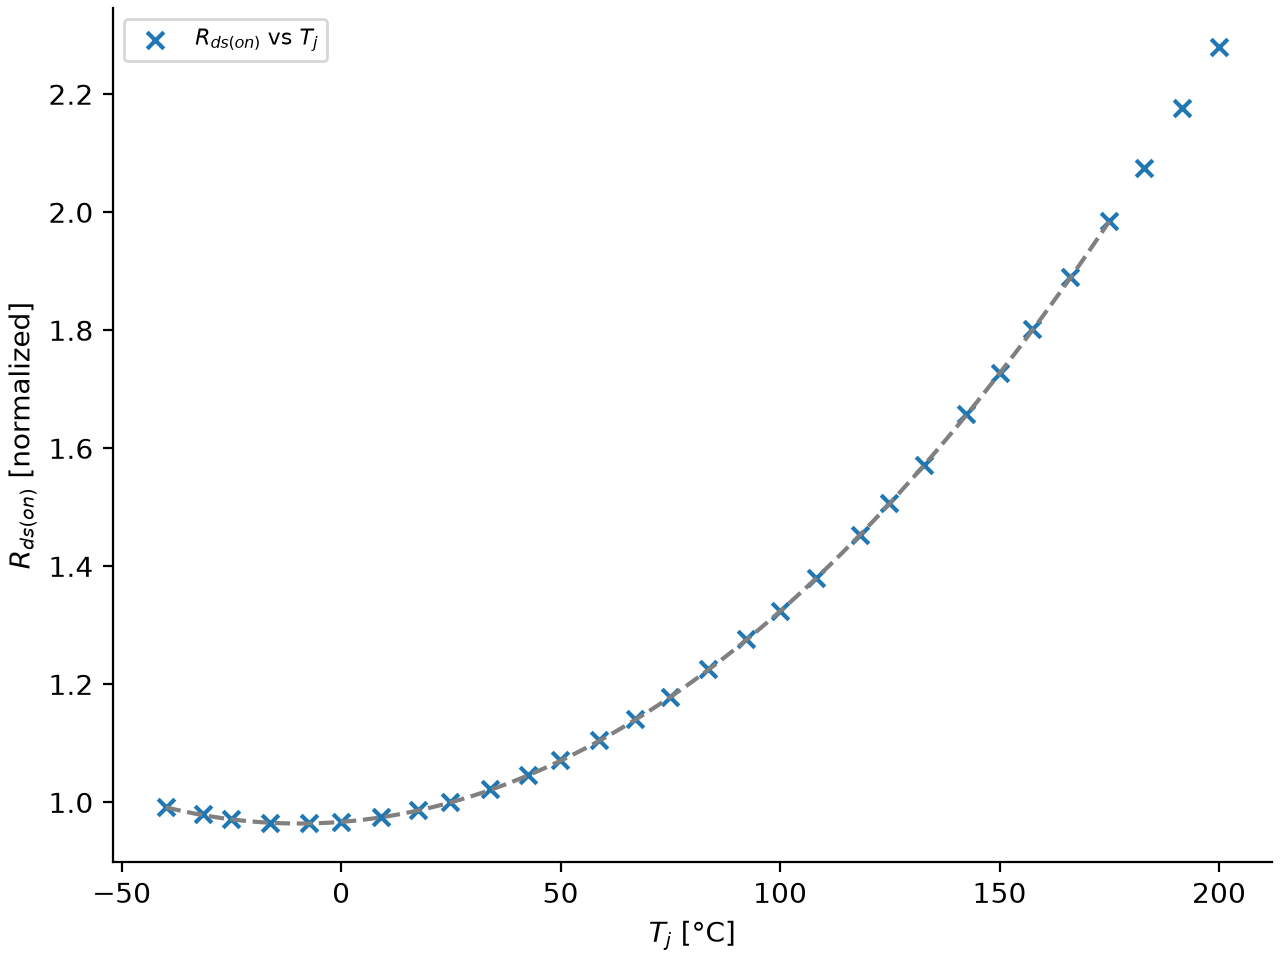
\includegraphics[width=0.48\linewidth]{figures/inputs/Rdson_vs_Tj.png}\hfill
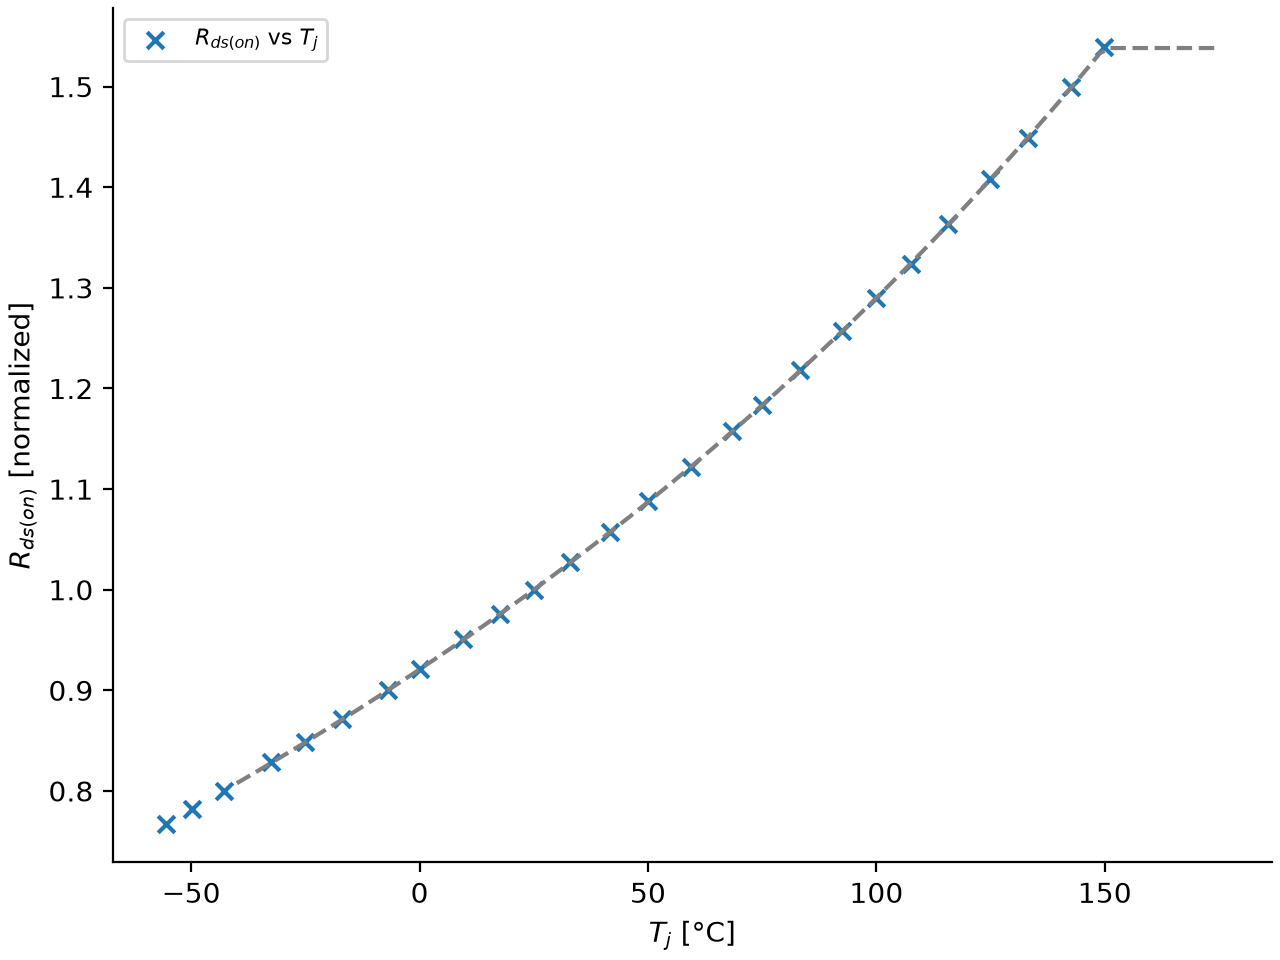
\includegraphics[width=0.48\linewidth]{figures/inputs/Rdson_vs_Tj_bimmc.png}
\caption{Normalised on-resistance versus junction temperature: datasheet points and cubic fit for the 2L SiC module (left) and the Si MOSFET of the BI-MMC (right).}
\label{fig:rdson}
\end{figure}

\paragraph{Battery loss.} The inverter input power is the electrical power of the machine terminals, $P_\mathrm{in}=\tfrac32(v_\mathrm{d}i_\mathrm{d}+v_\mathrm{q}i_\mathrm{q})$, written in the code as $\tfrac32\Ihat\,\hat v\cos(\angle v-\angle i)$. The DC current includes the converter losses, with the sign of the power flow, and the pack loss is the Joule loss in the series and parallel scaled cell resistances (the RC branch is at steady state for a constant current):
\begin{equation}
I_\mathrm{dc}=\frac{P_\mathrm{in}+\operatorname{sgn}(P_\mathrm{in})\,(P_\mathrm{c}+P_\mathrm{s})}{V_\mathrm{dc}(z)},\qquad
P_\mathrm{b}^\mathrm{2L}=I_\mathrm{dc}^2\,(R_0+R_1)\,\frac{N_\mathrm{s}}{N_\mathrm{p}}.
\label{eq:pb2l}
\end{equation}
The DC-link ripple current and the capacitor are not modelled.

\subsection{BI-MMC losses}\label{sec:lossbimmc}
\code{calc.calc_losses_bimmc} has the same inputs and outputs as the 2L function. The converter has $3\Nsm$ SMs with four switches each.

\paragraph{Conduction loss.} In a full-bridge SM the current always flows through two series devices, in the inserted states as well as in the bypass state. The RMS value of a device current is $\Ihat/(\sqrt2N_\mathrm{p,mos})$, so one SM dissipates $2\cdot\tfrac12\Ihat^2\Rds/N_\mathrm{p,mos}$ and the converter
\begin{equation}
P_\mathrm{c}^\mathrm{BI}=3\,\Nsm\,\Rds\,\frac{i_\mathrm{d}^2+i_\mathrm{q}^2}{N_\mathrm{p,mos}}.
\label{eq:pcbimmc}
\end{equation}
It is evaluated with the same fixed-point iteration on $\Rds(\Tj)$ as the 2L drive (\cref{eq:rdsiter}) using the Infineon polynomial.

\paragraph{Switching loss.} The BI-MMC uses the same slope-based scheme, with the SM voltage $v_\mathrm{s}=\Nssm V_\mathrm{cell}(z)$ in place of $V_\mathrm{dc}$ in the voltage intervals of \cref{eq:times}, and constant slopes ($\SI{1}{\ampere\per\nano\second}$ and $\SI{0.5}{\volt\per\nano\second}$ by default). All $4\Nsm$ switches of a phase are assumed to switch once per carrier period, at the frequency $f_\mathrm{c}=m_\mathrm{f}\,p\,\omega_\mathrm{m}/(2\pi)$:
\begin{equation}
E_\mathrm{sw}=\tfrac12v_\mathrm{s}\,\bar\imath\,\big(t_\mathrm{ri}+t_\mathrm{fv}+t_\mathrm{fi}+t_\mathrm{rv}\big),\qquad
P_\mathrm{s}^\mathrm{BI}=3\cdot4\Nsm\,E_\mathrm{sw}\,f_\mathrm{c}.
\label{eq:psbimmc}
\end{equation}

\paragraph{Temperatures.} Analogous to \cref{eq:thermal2l}, with $P_\mathrm{dev}=(P_\mathrm{c}+P_\mathrm{s})/(3\Nsm\cdot4N_\mathrm{p,mos})$ and the thermal resistances of the BI-MMC devices (\SI{0.5}{\kelvin\per\watt} junction-to-case, \SI{0.2}{\kelvin\per\watt} case-to-ambient by default).

\paragraph{Battery loss from the gated phase current.} The cells of an SM carry the phase current while the SM is inserted. For each operating point the code simulates two electrical periods in the time domain with $\theta=\omega_\mathrm{e}t$:
\begin{align}
i_\mathrm{o}(\theta)&=i_\mathrm{d}\cos\theta-i_\mathrm{q}\sin\theta, \label{eq:io}\\
v_\mathrm{ref}(\theta)&=\frac{v_\mathrm{d}\cos\theta-v_\mathrm{q}\sin\theta}{v_\mathrm{s}\,\Nsm\,(1-r)}, \label{eq:vref}\\
g_1&=\big[v_\mathrm{ref}>c(t)\big],\quad g_3=\big[v_\mathrm{ref}<-c(t)\big],\quad s=g_1-g_3\in\{-1,0,1\},\label{eq:gate}\\
i_\mathrm{b}(t)&=g_1\,i_\mathrm{o}-g_3\,i_\mathrm{o}=s(t)\,i_\mathrm{o}(t), \label{eq:ib}
\end{align}
where $c(t)\in[-1,1]$ is a symmetric triangular carrier of frequency $f_\mathrm{c}$ (\code{scipy.signal.sawtooth} with width $0.5$). This is unipolar PWM with a single carrier. All SMs of a phase are assumed to carry the same $s(t)$, so the result of one SM is multiplied by $3\Nsm$. \Cref{fig:pwm} shows one period of these signals. The SM cell string is the equivalent circuit of \cref{sec:sizing}, scaled to $\Nssm$ series and $\Npsm$ parallel cells:
\begin{equation}
R_{0}'=R_0\frac{\Nssm}{\Npsm},\quad R_{1}'=R_1\frac{\Nssm}{\Npsm},\quad C_{1}'=C_1\frac{\Npsm}{\Nssm},
\label{eq:smrc}
\end{equation}
and its state and loss are
\begin{equation}
\frac{\mathrm{d}v_C}{\mathrm{d}t}=\frac{1}{C_1'}\Big(i_\mathrm{b}-\frac{v_C}{R_1'}\Big),\qquad
p_\mathrm{b}(t)=R_0'i_\mathrm{b}^2+\frac{v_C^2}{R_1'}.
\label{eq:rcsim}
\end{equation}
\Cref{eq:rcsim} is integrated with explicit Euler and a step $\Delta t=1/(100f_\mathrm{c})$ (\code{calc.simulate_battery_loss}, compiled with Numba). The first electrical period lets $v_C$ settle and is discarded; the loss is the mean of $p_\mathrm{b}$ over the second period, and the total battery loss is
\begin{equation}
P_\mathrm{b}^\mathrm{BI}=3\,\Nsm\,\big\langle p_\mathrm{b}\big\rangle_{T_\mathrm{e}}.
\label{eq:pbbimmc}
\end{equation}
Explicit Euler with this step is stable only for electrical frequencies above about \SI{8}{\hertz}; the model therefore needs $\omega_\mathrm{e}>0$. On the map grid, the standstill column of the BI-MMC is left empty (NaN); the cycle evaluation applies a speed floor (\cref{sec:cycles}).

\begin{figure}[ht]
\centering
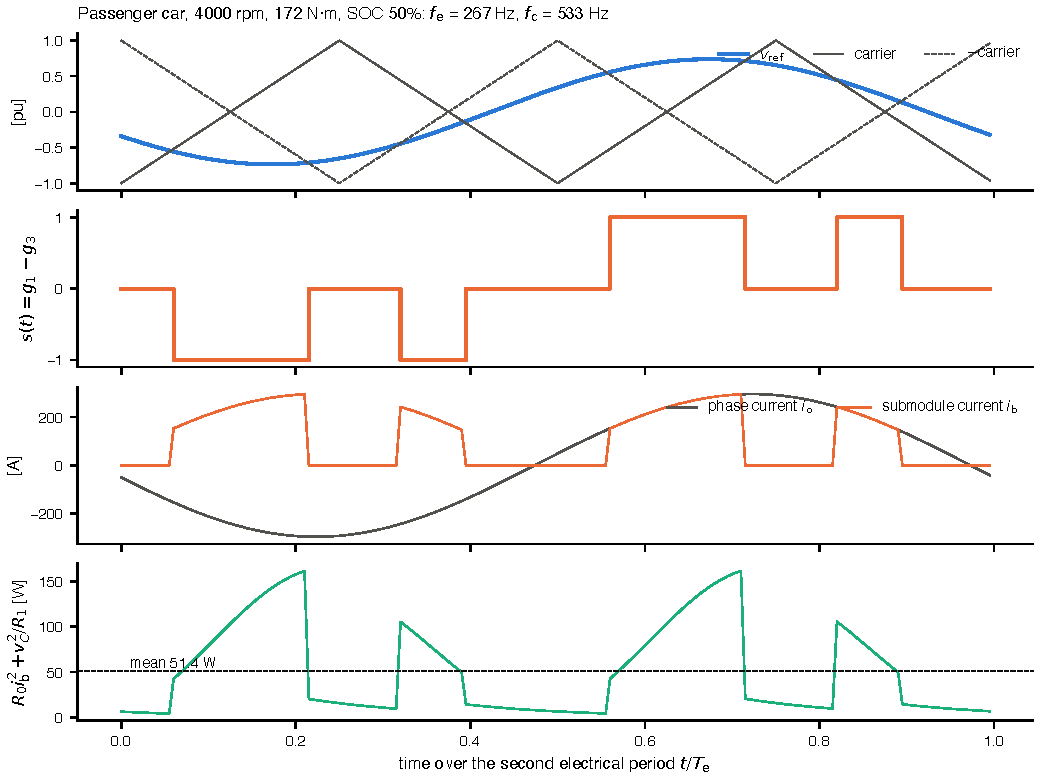
\includegraphics[width=0.85\linewidth]{figures/paper_pwm.pdf}
\caption{BI-MMC battery-loss simulation for one operating point (passenger car): reference and carrier, gating state $s=g_1-g_3$, phase current $i_\mathrm{o}$ and submodule current $i_\mathrm{b}=s\,i_\mathrm{o}$, and instantaneous cell loss. The figure is produced with the equations of the text and checked against \code{calc.simulate_battery_loss}.}
\label{fig:pwm}
\end{figure}

\subsection{Efficiency definitions}\label{sec:effdef}
\paragraph{Operating-point efficiency.} The shaft power is $P_\mathrm{out}=\omega_\mathrm{m}T$, positive in motoring and negative in regeneration, and the total loss is $P_\mathrm{loss}=P_\mathrm{c}+P_\mathrm{s}+P_\mathrm{b}$ (\code{model.efficiency}):
\begin{equation}
\eta=\frac{P_\mathrm{out}}{P_\mathrm{out}+\operatorname{sgn}(P_\mathrm{out})\,P_\mathrm{loss}}.
\label{eq:eta}
\end{equation}
In motoring this is the usual shaft power over input power. In regeneration, \cref{eq:eta} gives $|P_\mathrm{out}|/(|P_\mathrm{out}|+P_\mathrm{loss})$, which stays below \SI{100}{\percent} and equals $1-P_\mathrm{loss}/|P_\mathrm{out}|$ to first order. The efficiency of a single component $k\in\{\mathrm{c},\mathrm{s},\mathrm{b}\}$ is $\eta_k=\eta(P_\mathrm{out},P_k)$. Machine losses are not included.

\paragraph{Cycle efficiency.} For a duty cycle, the efficiency is energy based (\cref{eq:etacyc} in \cref{sec:cycles}).

\section{Analysis I: Efficiency Maps}\label{sec:maps}
The first analysis answers the question \emph{where in the torque--speed plane is each drive more efficient?} It evaluates \cref{eq:mtpa,eq:pc2l,eq:ps2l,eq:pb2l,eq:pcbimmc,eq:psbimmc,eq:pbbimmc,eq:eta} on a fixed grid at a given SOC. It is implemented in \code{model.loss_maps} and driven by \code{main.py} (interactive) or \code{create_maps_PCIM.py} (all applications).

\subsection{Method}
\paragraph{Grid.} The default grid (\code{model.default_grid}) has 50 speeds, $\omega_\mathrm{m}\in[0,\omega_\mathrm{m,max}]$, and 100 torques, $T\in[-T_\mathrm{b},T_\mathrm{b}]$, so that motoring ($T>0$) and regeneration ($T<0$) are covered. The shaft power on the grid is $P_\mathrm{out}=\omega_\mathrm{m}T$.

\paragraph{Operating envelope.} A grid point belongs to the map of a drive if (i)~$|P_\mathrm{out}|\le P_\mathrm{b}$, (ii)~the MTPA problem \cref{eq:mtpa} has a solution under the drive's voltage limit \cref{eq:vmax}, and (iii)~$i_\mathrm{d}^2+i_\mathrm{q}^2\le I_\mathrm{b}^2$. All other points are NaN. The envelope of the drive with the lower voltage limit is therefore smaller at high speed, and low SOC shrinks both envelopes.

\paragraph{Algorithm.} \Cref{alg:maps} lists the steps. The loss functions receive whole arrays, so each of the two drives is evaluated with one call; only the BI-MMC battery loss needs a loop over the grid because of the time-domain simulation.

\begin{lstlisting}[caption={Efficiency maps (\code{model.loss_maps}) at a given SOC $z$.}, label={alg:maps}]
d  $\leftarrow$ design(p);  (V$_\mathrm{cell}$, R$_0$, R$_1$, C$_1$) $\leftarrow$ cell_state(p, z)
V$_\mathrm{dc}$ $\leftarrow$ V$_\mathrm{cell}$ N$_\mathrm{s}$;   $\hat v^\mathrm{2L}_\mathrm{max}$ $\leftarrow$ V$_\mathrm{dc}$/$\sqrt3$;   $v_\mathrm{s}$ $\leftarrow$ V$_\mathrm{cell}$ N$_\mathrm{s,sm}$
$\hat v^\mathrm{BI}_\mathrm{max}$ $\leftarrow$ $v_\mathrm{s}$ N$_\mathrm{sm}$ (1-r)      // "own"; equal to $\hat v^\mathrm{2L}_\mathrm{max}$ for the dashboard setting
for each drive X in {2L, BI-MMC}:
    for each speed $\omega_\mathrm{m}$ (outer) and torque T (inner):
        if |$\omega_\mathrm{m}$ T| > P$_\mathrm{b}$: mark NaN; continue
        solve Eq. $\eqref{eq:mtpa}$ with limit $\hat v^X_\mathrm{max}$, warm start from the last solution
        if the solver fails or i$_\mathrm{d}^2$+i$_\mathrm{q}^2$ > I$_\mathrm{b}^2$: mark NaN
    (v$_\mathrm{d}$, v$_\mathrm{q}$) $\leftarrow$ Eq. $\eqref{eq:vd}$, $\eqref{eq:vq}$ for X's currents
(P$_\mathrm{c}$, P$_\mathrm{s}$, P$_\mathrm{b}$, T$_\mathrm{j}$, T$_\mathrm{c}$) of 2L $\leftarrow$ 5 x calc_losses_2l with R$_\mathrm{ds,on}$ iteration, Eq. $\eqref{eq:rdsiter}$
f$_\mathrm{c}$ $\leftarrow$ m$_\mathrm{f}$ p $\omega_\mathrm{m}$/(2$\pi$)
(P$_\mathrm{c}$, P$_\mathrm{s}$, P$_\mathrm{b}$, T$_\mathrm{j}$, T$_\mathrm{c}$) of BI-MMC $\leftarrow$ calc_losses_bimmc, battery loss from Eq. $\eqref{eq:io}$-$\eqref{eq:pbbimmc}$
T$_\mathrm{cell}$ $\leftarrow$ Eq. $\eqref{eq:tcell}$ for both drives
$\eta$ $\leftarrow$ Eq. $\eqref{eq:eta}$;  $\Delta\eta$ $\leftarrow$ $\eta^\mathrm{BI}$ - $\eta^\mathrm{2L}$
\end{lstlisting}

\paragraph{Settings.} \code{loss_maps} has two switches. With \code{voltage_limit="own"} (default) each drive uses its own limit; \code{"2l"} gives the 2L limit to both, as the original dashboard does. With \code{rdson_tj=True} (default) $\Rds$ follows $\Tj$ for both drives; \code{False} keeps the \SI{25}{\celsius} value. All maps of this paper use the defaults.

\paragraph{Thermal limits.} The result also holds the steady-state flags $\Tj\le T_\mathrm{j,max}$ and $\Tc\le T_\mathrm{c,max}$ (\SI{175}{\celsius} and \SI{100}{\celsius} for the 2L module; \SI{175}{\celsius} for the BI-MMC). The maps are \emph{not} masked by them, because a transient cycle can pass through such points without reaching steady state.

\subsection{Outputs}
For each drive the platform draws (i)~MTPA maps: $i_\mathrm{d}$, $i_\mathrm{q}$, $v_\mathrm{d}$, $v_\mathrm{q}$ in per unit of $I_\mathrm{b}$ and $V_\mathrm{dc}$, and the magnitudes and power factor; (ii)~loss maps $P_\mathrm{c}$, $P_\mathrm{s}$, $P_\mathrm{b}$ in kW; (iii)~temperature maps $\Tc$, $\Tj$, $T_\mathrm{cell}$; and (iv)~efficiency maps $\eta_\mathrm{c}$, $\eta_\mathrm{s}$, $\eta_\mathrm{b}$ and $\eta$, where values below $\SI{90}{\percent}$ are not drawn. For the comparison it draws the total loss and efficiency of both drives and their difference $\Delta\eta=\eta^\mathrm{BI}-\eta^\mathrm{2L}$ (blue: the BI-MMC is better), and the same difference for each loss component. All plotted data can be written to one Excel workbook. The red dashed line in all figures is the torque limit, $\min(T_\mathrm{b},P_\mathrm{b}/\omega_\mathrm{m})$.

\subsection{Reading the maps}
\Cref{fig:mapcar} shows the MTPA currents and voltages of the passenger car. Below base speed ($\SI{5000}{\rpm}$), $i_\mathrm{d}$ is only used for reluctance torque, and the voltage rises with speed. At and above base speed the voltage limit becomes active, $i_\mathrm{d}$ turns strongly negative (field weakening) and $i_\mathrm{q}$ falls so that the torque follows the constant-power limit. It is this region where the two drives differ most, because the field-weakening current is a reactive current that flows through the cells of the BI-MMC but not through the cells of the 2L pack.

\begin{figure}[ht]
\centering
\includegraphics[width=0.78\linewidth]{figures/maps/car/mtpa_maps_soc_50.png}
\caption{MTPA currents and voltages of the passenger car at \SI{50}{\percent} SOC (per unit of $I_\mathrm{b}=\SI{500}{\ampere}$ and $V_\mathrm{dc}$). Red dashed line: torque limit.}
\label{fig:mapcar}
\end{figure}

\section{Analysis II: Drive-Cycle Efficiency}\label{sec:cycles}
The second analysis answers the question \emph{which drive uses less energy over a duty cycle?} It reuses the models of \cref{sec:models} unchanged, but instead of a fixed grid the operating points come from a time series, and the SOC and the temperatures evolve along it. It is implemented in \code{cycles.py} (cycle to machine profile) and \code{cycle_eval.py} (evaluation).

\subsection{From duty cycle to machine profile}\label{sec:profile}
Five kinds of cycle are supported. Each one returns the time $t$, the sample duration $\Delta t$, the machine speed $\omega_\mathrm{m}$ and the requested torque $T^*$ (\code{cycles.machine_profile}). \Cref{fig:profiles} shows the speed profiles.

\paragraph{Road-load model (car, bus, truck, train).} For a vehicle speed $v$ [\si{\metre\per\second}], acceleration $a$ and road slope $\alpha$, the tractive force at the wheel is (\code{applications.road_load_force})
\begin{equation}
F=k_\mathrm{m}\,m\,a+R(v,\alpha)+m\,g\sin\alpha,
\label{eq:roadload}
\end{equation}
with the rotating-mass factor $k_\mathrm{m}$; $R$ and the grade term are set to zero at standstill ($v\le\SI{0.01}{\metre\per\second}$), and
\begin{equation}
R=\begin{cases}\tfrac12\rho\,C_\mathrm{d}A\,v^2+\big(c_\mathrm{rr}+c_{\mathrm{rr},v}v\big)\,m\,g\cos\alpha & \text{road vehicles},\\[2pt] A_0+B_0v_\mathrm{kmh}+C_0v_\mathrm{kmh}^2 & \text{train (Davis)},\end{cases}\qquad R=0\ \text{if}\ v\le\SI{0.01}{\metre\per\second}.
\label{eq:resistance}
\end{equation}
With the wheel radius $r_\mathrm{w}$, gear ratio $G$ and gear efficiency $\eta_\mathrm{g}$, the machine speed and torque are (\code{cycles._wheel_to_machine})
\begin{equation}
\omega_\mathrm{m}=\frac{G\,v}{r_\mathrm{w}},\qquad
T^*=\begin{cases}\dfrac{F\,r_\mathrm{w}}{G\,\eta_\mathrm{g}} & F\ge0\ \text{(motoring)},\\[6pt] \dfrac{F\,r_\mathrm{w}\,\eta_\mathrm{g}}{G} & F<0\ \text{(regeneration)}.\end{cases}
\label{eq:wheel2machine}
\end{equation}
Gear losses are thus charged to the machine torque and are not part of the converter efficiency. \Cref{tab:vehicles} lists the vehicle data. Unless a gear ratio is given, it maps the top speed $v_\mathrm{top}$ to \SI{95}{\percent} of the maximum machine speed, $G=0.95\,\omega_\mathrm{m,max}r_\mathrm{w}/v_\mathrm{top}$ (\code{applications.gear_ratio}).

\begin{table}[ht]
\centering
\caption{Vehicle data of the road and rail applications ($m$ vehicle mass, $k_\mathrm{m}$ rotating-mass factor, $C_\mathrm{d}A$ drag area, $c_\mathrm{rr}$ rolling resistance, $r_\mathrm{w}$ wheel radius, $\eta_\mathrm{g}$ gear efficiency, $G$ gear ratio). The train uses the Davis coefficients $A_0=\SI{1000}{\newton}$, $B_0=\SI{10}{\newton\per(\kilo\metre\per\hour)}$, $C_0=\SI{0.10}{\newton\per(\kilo\metre\per\hour)\squared}$. The truck also has a speed-dependent rolling resistance $c_{\mathrm{rr},v}$ from the data file. Values are typical literature values (assumptions).}
\label{tab:vehicles}
\footnotesize
\begin{tabular}{@{}lrrrrrrr@{}}
\toprule
Application & $m$ [t] & $k_\mathrm{m}$ & $C_\mathrm{d}A$ [m$^2$] & $c_\mathrm{rr}$ & $r_\mathrm{w}$ [m] & $\eta_\mathrm{g}$ & $G$ \\
\midrule
Passenger car & 1.9 & 1.05 & 0.62 & 0.0085 & 0.33 & 0.97 & 8.4 \\
City bus & 15.0 & 1.08 & 5.00 & 0.007 & 0.48 & 0.96 & 19.0 \\
Heavy-duty truck & 40.0 & 1.00 & 5.00 & 0.006 & 0.50 & 0.96 & 10.6 \\
Off-road machine & \multicolumn{7}{c}{normalised / mode-based cycle, no vehicle model} \\
Marine vessel & \multicolumn{7}{c}{normalised / mode-based cycle, no vehicle model} \\
Regional train & 60.0 & 1.08 & Davis & -- & 0.43 & 0.97 & 5.6
\\
\bottomrule
\end{tabular}
\end{table}

\begin{figure}[ht]
\centering
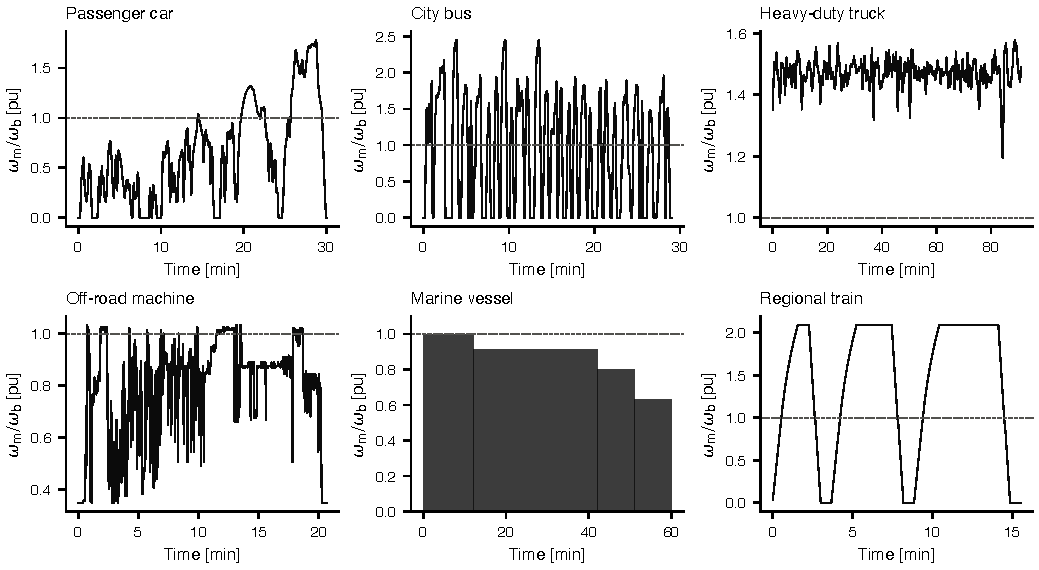
\includegraphics[width=\linewidth]{figures/paper_profiles.pdf}
\caption{Machine speed in per unit of base speed for the six duty cycles (dashed: base speed). Speed above 1 pu is field weakening.}
\label{fig:profiles}
\end{figure}

\paragraph{Speed cycles (car, bus).} The public speed traces WLTC Class~3b \cite{gtr15} and Braunschweig \cite{drivecat} (1~Hz, \code{data/cycles/}) give $v(t)$; the acceleration is the numerical gradient, $a=\mathrm{d}v/\mathrm{d}t$ (central differences), and \cref{eq:roadload,eq:wheel2machine} follow. The WHVC \cite{gtr4} is also in the data folder but is not used for the six presets.

\paragraph{Road cycle (truck).} The truck follows a measured road (distance and slope profile of the Södertälje--Norrköping route, \SI{119}{\kilo\metre}, from \code{so_no/}) under a proportional cruise controller. The longitudinal dynamics
\begin{equation}
\dot x=v,\qquad k_\mathrm{m}m\,\dot v=F_\mathrm{ctrl}-R\big(v,\alpha(x)\big)-mg\sin\alpha(x),\qquad
F_\mathrm{ctrl}=\operatorname{clip}\big(k_\mathrm{p}(v_\mathrm{set}-v),\pm F_\mathrm{max}\big)
\label{eq:cruise}
\end{equation}
are integrated with \code{scipy.integrate.solve_ivp} (RK45, output every \SI{1}{\second}) from $v_0=\SI{20}{\metre\per\second}$ until the end of the road, with $v_\mathrm{set}=\SI{80}{\kilo\metre\per\hour}$, $k_\mathrm{p}=\SI{e4}{\newton\per(\metre\per\second)}$ and $F_\mathrm{max}=\SI{7000}{\newton\metre}/r_\mathrm{w}$. Then $a$ is the gradient of $v(t)$, and \cref{eq:roadload,eq:wheel2machine} give the machine profile.

\paragraph{Normalised cycle (off-road machine).} The NRTC \cite{eu2017_654} gives speed in percent between idle and rated speed, and torque in percent of the maximum torque at that speed. With rated speed $\omega_\mathrm{r}=\omega_\mathrm{b}$ and idle speed $\omega_\mathrm{i}=0.35\,\omega_\mathrm{r}$,
\begin{equation}
\omega_\mathrm{m}=\omega_\mathrm{i}+\frac{n_\%}{100}(\omega_\mathrm{r}-\omega_\mathrm{i}),\qquad T^*=\frac{T_\%}{100}\min\Big(T_\mathrm{b},\frac{P_\mathrm{b}}{\omega_\mathrm{m}}\Big).
\label{eq:nrtc}
\end{equation}
The NRTC table contains no motoring (drag) points (see the README of \code{data/cycles/}); the code would treat such points as zero torque.

\paragraph{Mode cycle (marine vessel).} The ISO~8178 E3 propeller-law cycle \cite{iso8178_4} has four steady modes with speed $n_i=(1.00,0.91,0.80,0.63)$ pu, power $p_i=(1.00,0.75,0.50,0.25)$ pu and time weight $w_i=(0.20,0.50,0.15,0.15)$. With rated speed $\omega_\mathrm{b}$ and continuous rating $0.9P_\mathrm{b}$, mode $i$ lasts $w_i\cdot\SI{3600}{\second}$ at $\omega_{\mathrm{m},i}=n_i\omega_\mathrm{b}$ and $T_i^*=0.9\,p_iP_\mathrm{b}/\omega_{\mathrm{m},i}$.

\paragraph{Synthetic rail cycle (regional train).} A regional run with three station-to-station sections (\SIlist{4;7;10}{\kilo\metre}), a line speed of \SI{120}{\kilo\metre\per\hour}, maximum acceleration and deceleration of \SI{0.8}{\metre\per\second\squared} and \SI{40}{\second} dwell is generated with a time step of \SI{1}{\second} (\code{cycles.rail_cycle}). In each step the train brakes if the remaining distance is not larger than the braking distance $v^2/(2a_\mathrm{dec})$; otherwise it accelerates with
\begin{equation}
a=\min\Big(a_\mathrm{max},\ \frac{\min\big(F_\mathrm{lim},\,P_\mathrm{lim}/\max(v,0.1)\big)-R(v)}{k_\mathrm{m}m}\Big),\quad P_\mathrm{lim}=0.9P_\mathrm{b}\eta_\mathrm{g},\ \ F_\mathrm{lim}=\frac{0.9\,T_\mathrm{b}G\eta_\mathrm{g}}{r_\mathrm{w}},
\label{eq:rail}
\end{equation}
up to the line speed, and then cruises. Then \cref{eq:roadload,eq:wheel2machine} apply.

\subsection{Sample-by-sample evaluation}\label{sec:eval}
\Cref{alg:cycle} gives the algorithm of \code{cycle_eval.evaluate_cycle}. For each sample, the cell state, the voltage limits, the torque that both drives can deliver, the losses of both drives and the new SOC are computed.

\begin{lstlisting}[caption={Cycle evaluation (\code{cycle_eval.evaluate_cycle}) from initial SOC $z_0$.}, label={alg:cycle}]
d $\leftarrow$ design(p);  (t, $\Delta t$, $\omega_\mathrm{m}$, T*) $\leftarrow$ machine_profile(app);  $\omega_\mathrm{m}$ $\leftarrow$ clip($\omega_\mathrm{m}$, 0, $\omega_\mathrm{m,max}$)
z$_X$ $\leftarrow$ z$_0$ for X in {2L, BI};  n$_\mathrm{cells}^X$ $\leftarrow$ cells of each pack
for each sample k with ($\omega_\mathrm{m}$, T*, $\Delta t$):
    cell$_X$ $\leftarrow$ cell_state(p, z$_X$)
    if T* = 0 and $\omega_\mathrm{m}$ = 0: T $\leftarrow$ 0, all losses 0, temperatures = ambient, converter off
    else:
        $\hat v^X_\mathrm{max}$ $\leftarrow$ Eq. $\eqref{eq:vmax}$ with the OCV of cell$_X$
        T$_\mathrm{lim}$ $\leftarrow$ P$_\mathrm{b}$/$\omega_\mathrm{m}$ (1 - 10$^{-9}$);   T$_\mathrm{cmd}$ $\leftarrow$ clip(T*, -T$_\mathrm{lim}$, T$_\mathrm{lim}$)
        for X in {2L, BI}: (T$_X$, i$_X$) $\leftarrow$ feasible_torque(T$_\mathrm{cmd}$, $\hat v^X_\mathrm{max}$)       // Eq. $\eqref{eq:bisect}$
        T $\leftarrow$ sign(T$_\mathrm{cmd}$) min(|T$_\mathrm{2L}$|, |T$_\mathrm{BI}$|)                                // common torque
        for X with |T$_X$| $\neq$ |T|: i$_X$ $\leftarrow$ MTPA at the common torque T
        if some i$_X$ is None: mark sample infeasible, losses 0, T$_\mathrm{j}$ = T$_\mathrm{c}$ = NaN
        else: (P$_\mathrm{c}$, P$_\mathrm{s}$, P$_\mathrm{b}$, T$_\mathrm{j}$, T$_\mathrm{c}$)$_X$ $\leftarrow$ losses_2l / losses_bimmc
    P $\leftarrow$ $\omega_\mathrm{m}$ T;  T$_\mathrm{cell}^X$ $\leftarrow$ Eq. $\eqref{eq:tcell}$
    for X: I$_\mathrm{cell}^X$ $\leftarrow$ (P + P$_\mathrm{c}$ + P$_\mathrm{s}$ + P$_\mathrm{b}$) / (n$_\mathrm{cells}^X$ V$_\mathrm{cell}$);  z$_X$ $\leftarrow$ clip(z$_X$ - I$_\mathrm{cell}^X$ $\Delta t$ / (3600 Q$_\mathrm{cell}$), 0, 1)
accumulate energies and metrics, Eqs. $\eqref{eq:energies}$-$\eqref{eq:etacyc}$
\end{lstlisting}

\paragraph{Speed clipping and standstill.} The speed is limited to the range $[0,\omega_\mathrm{m,max}]$ (regeneration is represented by negative torque only). At standstill with zero torque the converters are off.

\paragraph{Common torque.} Both drives must deliver the same mechanical cycle, so that their efficiencies are comparable. The commanded torque is first limited by the rated power, $|T_\mathrm{cmd}|\le P_\mathrm{b}/\omega_\mathrm{m}$. If \cref{eq:mtpa} is infeasible at $T_\mathrm{cmd}$ for one of the drives (voltage or current limit), \code{feasible_torque} bisects the interval $[0,T_\mathrm{cmd}]$ ten times,
\begin{equation}
\text{keep the largest feasible } T\in[0,T_\mathrm{cmd}]\ \text{found by}\ T_{j+1}=\tfrac12(T_j^\mathrm{lo}+T_j^\mathrm{hi}),\ j=1\dots10,
\label{eq:bisect}
\end{equation}
which resolves the torque to $|T_\mathrm{cmd}|/2^{10}$. The delivered torque is the \emph{smaller} of the two drives' feasible torques, so neither drive gets an unfair advantage. The remainder, $T^*-T$, is assumed to be taken by the mechanical brake (regeneration) or not delivered (motoring) and is reported as ``clipped'' energy.

\paragraph{BI-MMC speed floor.} The time-domain battery simulation needs an electrical period and a stable step (\cref{sec:lossbimmc}). For low speeds, the BI-MMC loss is therefore evaluated at the effective speed $\omega_\mathrm{m,eff}=\max\big(\omega_\mathrm{m},\,2\pi f_\mathrm{c,min}/(m_\mathrm{f}p)\big)$ with $f_\mathrm{c,min}=\SI{50}{\hertz}$ (i.e.\ $f_\mathrm{e}\ge\SI{25}{\hertz}$ for $m_\mathrm{f}=2$), for the voltages, the carrier frequency (and hence switching and battery loss) and the gating, while the currents and the torque are those of the actual operating point. This floor makes the BI-MMC loss at creep speed an estimate, not an exact value.

\paragraph{State of charge.} Each pack is a power source at its OCV. The power drawn from it is the mechanical power plus the total loss (the cell resistance loss is part of $P_\mathrm{b}$), shared equally by the $n_\mathrm{cells}$ cells ($N_\mathrm{s}N_\mathrm{p}$ for the 2L pack, $3\Nsm\Nssm\Npsm$ for the BI-MMC):
\begin{equation}
I_\mathrm{cell}=\frac{P+P_\mathrm{c}+P_\mathrm{s}+P_\mathrm{b}}{n_\mathrm{cells}V_\mathrm{cell}(z_k)},\qquad
z_{k+1}=\operatorname{clip}\Big(z_k-\frac{I_\mathrm{cell}\Delta t}{3600\,Q_\mathrm{cell}},\,0,\,1\Big).
\label{eq:soc}
\end{equation}
The two drives therefore follow slightly different SOC trajectories, and the voltage limit and the cell parameters are updated at every step.

\paragraph{Thermal state.} Junction, case and cell temperatures are the \emph{steady-state} values of \cref{eq:thermal2l,eq:tcell} for the loss of the present sample. There is no thermal capacitance, so the peak temperatures are upper bounds for samples shorter than the thermal time constants.

\subsection{Cycle metrics}\label{sec:metrics}
With $P_k=\omega_{\mathrm{m},k}T_k$ and the sample duration $\Delta t_k$, the energies are ($\lfloor x\rfloor^+=\max(x,0)$)
\begin{align}
E_\mathrm{mot}&=\sum_k\lfloor P_k\rfloor^+\Delta t_k, & E_\mathrm{reg}&=\sum_k\lfloor -P_k\rfloor^+\Delta t_k, \label{eq:energies}\\
E_x^X&=\sum_kP_{x,k}^X\Delta t_k\quad(x\in\{\mathrm{c},\mathrm{s},\mathrm{b}\}),& E_\mathrm{loss}^X&=E_\mathrm{c}^X+E_\mathrm{s}^X+E_\mathrm{b}^X. \label{eq:eloss}
\end{align}
The cycle efficiency charges the losses to the traction energy throughput, and the difference between the drives is given in percentage points (pp):
\begin{equation}
\etacyc^X=1-\frac{E_\mathrm{loss}^X}{E_\mathrm{mot}+E_\mathrm{reg}},\qquad
\Delta\etacyc=\etacyc^\mathrm{BI}-\etacyc^\mathrm{2L}.
\label{eq:etacyc}
\end{equation}
Further outputs are the net battery energy $E_\mathrm{mot}-E_\mathrm{reg}+E_\mathrm{loss}$ (per \SI{100}{\kilo\metre} for vehicle cycles), the relative loss change $E_\mathrm{loss}^\mathrm{BI}/E_\mathrm{loss}^\mathrm{2L}-1$, the final SOC, the peak temperatures, the clipped energies in motoring and regeneration, $\sum\big(\lfloor P^*\rfloor^+-\lfloor P\rfloor^+\big)\Delta t$ and $\sum\big(\lfloor -P^*\rfloor^+-\lfloor -P\rfloor^+\big)\Delta t$ with $P^*=\omega_\mathrm{m}T^*$, and the share of mechanical energy delivered below base speed,
\begin{equation}
\sigma_\mathrm{b}=\frac{\sum_k|P_k|\Delta t_k\,[\omega_{\mathrm{m},k}\le\omega_\mathrm{b}]}{\sum_k|P_k|\Delta t_k},
\label{eq:share}
\end{equation}
which will turn out to be the best predictor of $\Delta\etacyc$ (\cref{sec:results}). \Cref{eq:etacyc} differs from the point efficiency \cref{eq:eta}: it weights each operating point by the energy processed there, which is what a drive cycle requires.

\paragraph{Relation to the maps.} \Cref{eq:etacyc} is the energy-weighted mean of the loss maps along the cycle, apart from three effects that the maps do not have: the SOC changes along the cycle, the common torque is limited by the weaker drive, and the BI-MMC speed floor. The cycle evaluation therefore does not interpolate the maps. The map backgrounds in \cref{sec:results} are used only to visualise where the cycle energy lies.

\section{Results for Six Applications}\label{sec:results}
The platform is applied to six applications with the same cell, the same device families and the same per-unit machine; they differ in rating, voltage, installed energy and duty (\cref{tab:machine,tab:conv,tab:cycles}). All results use the settings of \cref{sec:software} (BI-MMC sized by \cref{eq:npsm}, own voltage limit, $\Rds(\Tj)$) and \SI{50}{\percent} SOC unless stated otherwise. The vehicle parameters and the truck road data are assumptions (typical literature values or the data of an earlier study) and are not validated against measurements, so the results show trends and should not be read as predictions for a specific vehicle.

\begin{table}[ht]
\centering
\caption{Duty cycles of the six applications as processed by the code (\SI{50}{\percent} SOC, delivered mechanical power). $\sigma_\mathrm{b}$: share of the mechanical energy delivered below base speed; clipped: energy beyond the torque envelope assigned to the brake (regeneration) or not delivered (motoring).}
\label{tab:cycles}
\footnotesize
\setlength\tabcolsep{3pt}
\begin{tabular}{@{}llrrrrrrrrrr@{}}
\toprule
Application & Cycle & $t$ & Dist. & $G$ & $E_\mathrm{mot}$ & $E_\mathrm{reg}$ & $\max P$ & $\min P$ & $\sigma_\mathrm{b}$ & \multicolumn{2}{c}{Clipped [kWh]} \\
 & & [min] & [km] & [--] & [kWh] & [kWh] & [kW] & [kW] & [\%] & mot. & reg. \\
\midrule
Passenger car & WLTC Class 3b & 30.0 & 23.3 & 8.4 & 3.6 & 1.2 & 50 & -39 & 62 & 0.00 & 0.00 \\
City bus & Braunschweig & 29.0 & 10.9 & 19.0 & 13.8 & 8.7 & 174 & -318 & 26 & 0.00 & 0.00 \\
Heavy-duty truck & Södertälje--Norrköping & 90.9 & 118.9 & 10.6 & 159.0 & 24.8 & 475 & -261 & 0 & 0.00 & 0.00 \\
Off-road machine & NRTC & 20.6 & -- & -- & 17.2 & 0.0 & 150 & 0 & 79 & 0.00 & 0.00 \\
Marine vessel & ISO 8178 E3 & 60.0 & -- & -- & 247.5 & 0.0 & 360 & 90 & 100 & 0.00 & 0.00 \\
Regional train & Synthetic regional run & 15.6 & 21.0 & 5.6 & 49.0 & 16.1 & 548 & -600 & 19 & 0.08 & 11.46
\\
\bottomrule
\end{tabular}
\end{table}

\subsection{Analysis I: efficiency maps}
\Cref{fig:eta_car} shows the efficiency maps of the passenger car. Both drives reach peak efficiencies above \SI{99.7}{\percent} (\cref{tab:mapstats}; converter and battery only). The difference map divides the plane into three regions. (i)~At low speed and low to medium torque the BI-MMC is better, by up to a few percentage points near standstill, where the 2L inverter's switching loss at a fixed \SI{10}{\kilo\hertz} dominates while the BI-MMC switches at a multiple of a very low fundamental frequency. (ii)~Over most of the constant-torque region, the two drives are within a few tenths of a percentage point of each other; towards high torque the BI-MMC falls behind, because the battery loss grows with $\Ihat^2$ in both drives but with a larger factor in the BI-MMC. (iii)~Above base speed, the BI-MMC is clearly worse, by up to \SI{13}{\pp} at light load and high speed. There the 2L pack current $I_\mathrm{dc}$ stays small, whereas the field-weakening current flows through every inserted cell of the BI-MMC.

\begin{figure}[ht]
\centering
\includegraphics[width=0.8\linewidth]{figures/maps/car/efficiency_maps_comparison_soc_50.png}
\caption{Total efficiency (converter and battery) of the 2L inverter (top) and the BI-MMC (middle) and their difference $\Delta\eta$ (bottom; negative contours dashed) for the passenger car at \SI{50}{\percent} SOC. Values below \SI{90}{\percent} are not drawn.}
\label{fig:eta_car}
\end{figure}

\Cref{fig:loss_car} shows the three loss components separately as the difference 2L $-$ BI-MMC (blue: the BI-MMC has lower losses). In this application the BI-MMC wins in conduction everywhere, because \SI{0.3}{\milli\ohm} Si devices replace \SI{4.6}{\milli\ohm} SiC devices despite the two devices in series per SM, and it wins in switching everywhere, because of the low SM voltage and the low carrier frequency. The battery loss, however, is higher in the BI-MMC over the whole map, and it dominates in field weakening. At higher current and with more series SMs the conduction advantage disappears (see the truck and train below).

\begin{figure}[ht]
\centering
\includegraphics[width=0.8\linewidth]{figures/maps/car/individual_losses_maps_comparison_soc_50.png}
\caption{Loss difference 2L $-$ BI-MMC (in kW) per component for the passenger car at \SI{50}{\percent} SOC: conduction (top), switching (middle), battery (bottom). Blue: BI-MMC better; red: 2L better.}
\label{fig:loss_car}
\end{figure}

\begin{table}[ht]
\centering
\caption{Statistics of the efficiency maps at \SI{50}{\percent} SOC (50$\times$100 grid, points feasible for both drives with $|T|>2\,\%\,T_\mathrm{b}$). $\hat\eta$: peak efficiency; ``better'': share of grid points where the BI-MMC is more efficient; $\overline{\Delta\eta}$: mean efficiency difference BI-MMC $-$ 2L, below and above base speed; last two columns: largest and smallest $\Delta\eta$.}
\label{tab:mapstats}
\footnotesize
\setlength\tabcolsep{4pt}
\begin{tabular}{@{}lrrrrrrrr@{}}
\toprule
 & $\hat\eta^\mathrm{2L}$ & $\hat\eta^\mathrm{BI}$ & \multicolumn{2}{c}{$\omega_\mathrm{m}\le\omega_\mathrm{b}$} & \multicolumn{2}{c}{$\omega_\mathrm{m}>\omega_\mathrm{b}$} & max & min \\
Application & [\%] & [\%] & better [\%] & $\overline{\Delta\eta}$ [pp] & better [\%] & $\overline{\Delta\eta}$ [pp] & [pp] & [pp] \\
\midrule
Passenger car & 99.81 & 99.87 & 34 & +0.05 & 9 & -1.21 & +4.2 & -13.0 \\
City bus & 99.79 & 99.92 & 59 & +0.43 & 15 & -0.57 & +4.5 & -6.9 \\
Heavy-duty truck & 99.78 & 99.88 & 36 & -0.02 & 3 & -1.11 & +4.0 & -11.3 \\
Off-road machine & 99.80 & 99.94 & 100 & +0.77 & 67 & -0.10 & +5.8 & -3.1 \\
Marine vessel & 99.80 & 99.95 & 100 & +0.71 & 88 & +0.12 & +4.7 & -1.2 \\
Regional train & 99.74 & 99.85 & 23 & -0.48 & 3 & -1.62 & +3.9 & -16.1
\\
\bottomrule
\end{tabular}
\end{table}

\Cref{tab:mapstats} and \cref{fig:eta_two} give the picture for the other applications. In the off-road machine and the marine vessel, the BI-MMC is better at \emph{every} point below base speed, and above base speed it stays close (mean $-0.10$ and $+0.12$~pp). In the car, truck and train it wins only in small regions at low speed (\SIrange{23}{36}{\percent} of the sub-base map) and loses \SIrange{1.1}{1.6}{\pp} on average above base speed, with local losses up to \SI{16}{\pp} in the train and \SI{13}{\pp} in the car. The maps of the other applications are in \cref{app:traces}.

\begin{figure}[ht]
\centering
\includegraphics[width=0.49\linewidth]{figures/maps/offroad/efficiency_maps_comparison_soc_50.png}\hfill
\includegraphics[width=0.49\linewidth]{figures/maps/truck/efficiency_maps_comparison_soc_50.png}
\caption{Efficiency of the 2L inverter, the BI-MMC and their difference for the off-road machine (left) and the heavy-duty truck (right) at \SI{50}{\percent} SOC.}
\label{fig:eta_two}
\end{figure}

The temperature maps show that the thermal stress is small at the nominal ambient of \SI{25}{\celsius}. In the passenger car, the steady-state junction temperature peaks at about \SI{26}{\celsius} in the BI-MMC and at about \SI{38}{\celsius} in the 2L inverter, and the cell temperature rises by at most \SI{1.3}{\kelvin} in either drive (\cref{fig:tempcar}). The distribution of the loss over many devices keeps the BI-MMC junctions close to the ambient temperature, a side benefit that the efficiency maps do not show.

\begin{figure}[ht]
\centering
\includegraphics[width=0.49\linewidth]{figures/maps/car/temperature_maps_2l_soc_50.png}\hfill
\includegraphics[width=0.49\linewidth]{figures/maps/car/temperature_maps_bimmc_soc_50.png}
\caption{Steady-state case, junction and cell temperatures of the 2L inverter (left) and the BI-MMC (right), passenger car, \SI{50}{\percent} SOC.}
\label{fig:tempcar}
\end{figure}

\subsection{Analysis II: drive cycles}
\Cref{fig:delta_maps} places the cycle energy on the difference maps. Where the large dots lie in blue regions, the BI-MMC gains; red regions are lost. The off-road machine and the ship operate in the blue sub-base region. The car, bus and truck have much of their energy in light-red or red regions, and the train spends the largest dots in the field-weakening region where the difference exceeds $-4$~pp.

\begin{figure}[ht]
\centering
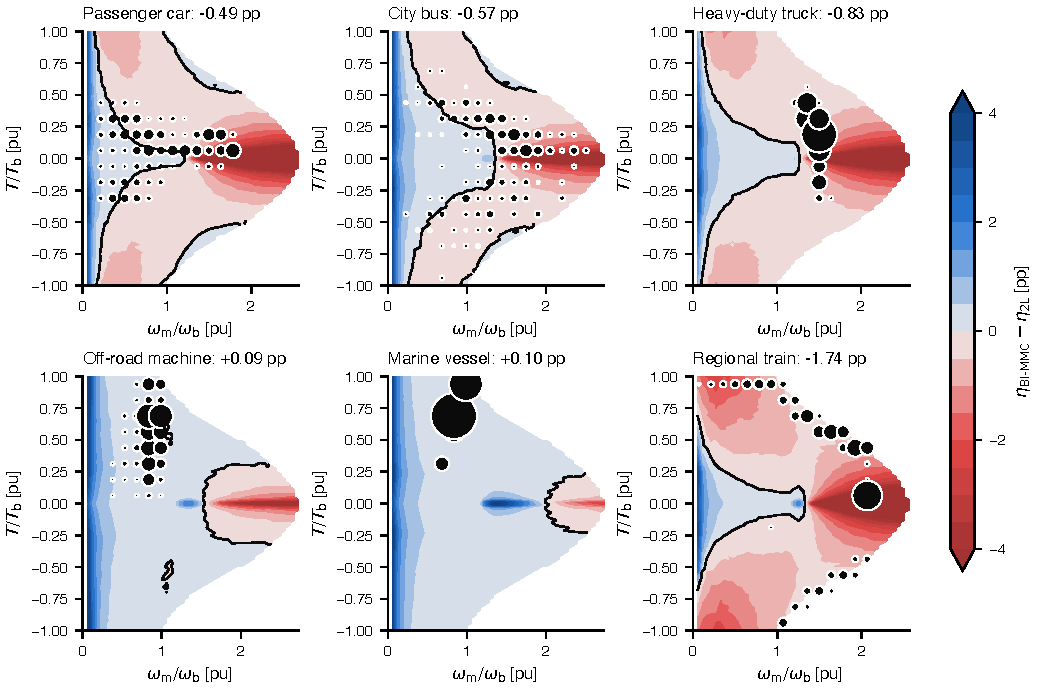
\includegraphics[width=\linewidth]{figures/paper_delta_maps.pdf}
\caption{Efficiency difference BI-MMC $-$ 2L over the torque--speed map at \SI{50}{\percent} SOC for the six applications (colour scale clipped to $\pm4$~pp). Dots: cycle energy $|P|\Delta t$ per bin; dot area is proportional to the energy share. Solid line: $\Delta\eta=0$. The title gives the cycle result $\Delta\etacyc$.}
\label{fig:delta_maps}
\end{figure}

\Cref{tab:ratios} and \cref{fig:summary} summarise the cycle results; \cref{tab:resfull} in the appendix lists the loss energies for all SOC values, and \cref{fig:trace_car,fig:trace_truck} (and the appendix) show the time series.

\begin{table}[ht]
\centering
\caption{Cycle results at \SI{50}{\percent} initial SOC. Semi.\ cut: reduction of semiconductor (conduction + switching) loss energy by the BI-MMC; $E_\mathrm{b}$ ratio: BI-MMC over 2L battery loss energy; $\Delta E_\mathrm{loss}$: relative change of the total loss energy; Cons.: net battery energy per \SI{100}{\kilo\metre} (2L, BI-MMC); $z_\mathrm{end}$: final SOC (2L, BI-MMC).}
\label{tab:ratios}
\footnotesize
\setlength\tabcolsep{4pt}
\begin{tabular}{@{}lrrrrrrr@{}}
\toprule
 & Semi.\ cut & $E_\mathrm{b}$ ratio & $\Delta E_\mathrm{loss}$ & \multicolumn{2}{c}{Cons.\ [kWh/100 km]} & \multicolumn{2}{c}{$z_\mathrm{end}$ [\%]} \\
Application & [\%] & [--] & [\%] & 2L & BI & 2L & BI \\
\midrule
Passenger car & 60 & 4.1 & +43 & 10.6 & 10.7 & 46.8 & 47.0 \\
City bus & 56 & 4.4 & +35 & 50.2 & 51.4 & 48.5 & 48.4 \\
Heavy-duty truck & 37 & 3.0 & +54 & 115.2 & 116.5 & 15.6 & 15.6 \\
Off-road machine & 80 & 1.7 & -9 & -- & -- & 41.4 & 41.5 \\
Marine vessel & 53 & 1.6 & -11 & -- & -- & 24.9 & 25.0 \\
Regional train & 26 & 2.2 & +61 & 165.3 & 170.7 & 38.7 & 38.4
\\
\bottomrule
\end{tabular}
\end{table}

\begin{table}[ht]
\centering
\caption{Cycle efficiency at \SI{50}{\percent} SOC; the second block lists the peak steady-state temperatures along the cycle. $\Delta\etacyc=\etacyc^\mathrm{BI}-\etacyc^\mathrm{2L}$ with the range over \SIrange{20}{90}{\percent} initial SOC.}
\label{tab:etacyc}
\footnotesize
\setlength\tabcolsep{4pt}
\begin{tabular}{@{}lrrrcrrrrrr@{}}
\toprule
 & $\etacyc^\mathrm{2L}$ & $\etacyc^\mathrm{BI}$ & $\Delta\etacyc$ & range & \multicolumn{2}{c}{$\Tj^\mathrm{max}$ [\si{\celsius}]} & \multicolumn{2}{c}{$\Tc^\mathrm{max}$ [\si{\celsius}]} & \multicolumn{2}{c}{$T_\mathrm{cell}^\mathrm{max}$ [\si{\celsius}]} \\
Application & [\%] & [\%] & [pp] & [pp] & 2L & BI & 2L & BI & 2L & BI \\
\midrule
Passenger car & 98.87 & 98.38 & -0.49 & [-0.77, -0.34] & 31 & 25 & 27 & 25 & 25.1 & 25.3 \\
City bus & 98.35 & 97.78 & -0.57 & [-0.86, -0.48] & 50 & 27 & 35 & 25 & 25.2 & 25.3 \\
Heavy-duty truck & 98.45 & 97.62 & -0.83 & [-1.58, -0.48] & 44 & 28 & 32 & 26 & 25.4 & 25.5 \\
Off-road machine & 99.02 & 99.10 & +0.09 & [+0.02, +0.09] & 44 & 25 & 32 & 25 & 25.2 & 25.2 \\
Marine vessel & 99.06 & 99.17 & +0.10 & [+0.05, +0.11] & 48 & 26 & 34 & 25 & 25.0 & 25.1 \\
Regional train & 97.15 & 95.40 & -1.74 & [-2.34, -1.68] & 54 & 29 & 36 & 26 & 26.1 & 26.4
\\
\bottomrule
\end{tabular}
\end{table}

\begin{figure}[ht]
\centering
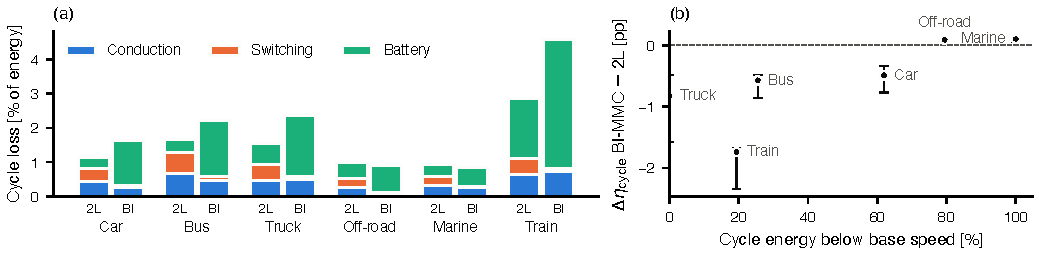
\includegraphics[width=\linewidth]{figures/cycle_summary.pdf}
\caption{(a) Cycle losses by component in percent of the traction energy throughput at \SI{50}{\percent} SOC; (b) cycle efficiency difference BI-MMC $-$ 2L versus the share $\sigma_\mathrm{b}$ of cycle energy below base speed (bars: \SIrange{20}{90}{\percent} SOC).}
\label{fig:summary}
\end{figure}

\paragraph{Where the losses go.} In every application, the BI-MMC cuts the semiconductor loss energy, by \SIrange{37}{80}{\percent} in car, bus, truck, off-road and marine duty and by \SI{26}{\percent} in the train (\cref{tab:ratios}). The saving comes mostly from switching, which almost vanishes (\cref{fig:summary}a). The conduction loss energy of the BI-MMC is lower in car, bus, off-road and marine duty (\SIrange{35}{81}{\percent} of the 2L value) but higher in the truck ($1.04\times$) and the train ($1.13\times$), where the high phase current flows through 11 and 13 series SMs (\cref{tab:resfull}). In exchange the battery loss energy is \numrange{1.6}{4.4} times higher. Because the battery loss is the largest component in all applications, the total loss energy of the BI-MMC is \SIrange{35}{61}{\percent} higher in car, bus, truck and train, and \SIrange{9}{11}{\percent} lower in the off-road machine and the ship. The net battery energy per \SI{100}{\kilo\metre} is correspondingly \SIrange{1.0}{3.3}{\percent} higher for the BI-MMC in the vehicle cycles. The peak junction temperature in the BI-MMC stays within \SI{4}{\kelvin} of the ambient, while the 2L inverter reaches \SIrange{31}{54}{\celsius}; this is a quasi-static estimate that overstates short peaks, and it is far from any limit for both drives.

\paragraph{Cycle efficiency and the share below base speed.} \Cref{fig:summary}b plots $\Delta\etacyc$ against $\sigma_\mathrm{b}$. The BI-MMC gains only when practically all cycle energy is delivered below base speed (marine vessel: $\sigma_\mathrm{b}=\SI{100}{\percent}$, $+0.10$~pp; off-road machine: \SI{79}{\percent}, $+0.09$~pp). Even then the gain is only about \SI{0.1}{\pp}. The truck ($\sigma_\mathrm{b}=0$, $-0.83$~pp) and the train (\SI{19}{\percent}, $-1.74$~pp) operate in field weakening and lose most. The passenger car and the city bus lose \SIrange{0.5}{0.6}{\pp}. The car has \SI{62}{\percent} of its energy below base speed, so $\sigma_\mathrm{b}$ alone is not sufficient: the car's light WLTC loads keep the 2L losses low, so the four-fold battery loss dominates. A low initial SOC lowers the cell voltage, deepens field weakening, and penalises the BI-MMC in all applications except the off-road machine and the ship, where the effect is within \SI{0.1}{\pp} (\cref{fig:soc}). The truck cycle ends at \SI{15.6}{\percent} SOC, so its late part is already in the low-SOC regime.

\begin{figure}[ht]
\centering
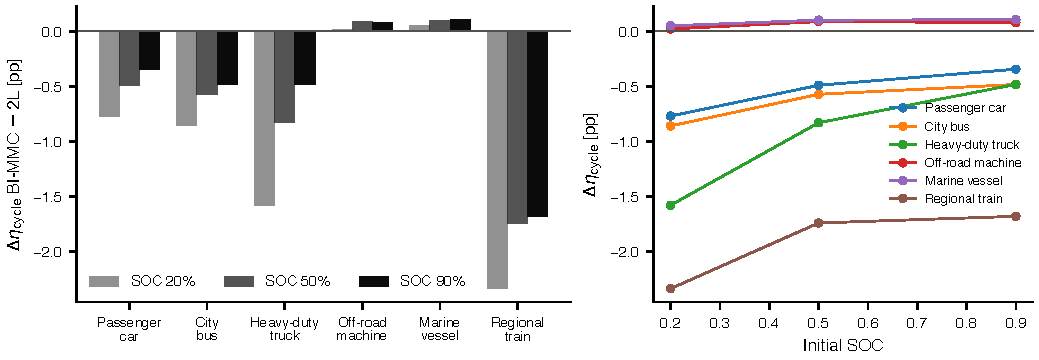
\includegraphics[width=\linewidth]{figures/paper_soc.pdf}
\caption{Cycle efficiency difference BI-MMC $-$ 2L for initial SOC of \SIlist{20;50;90}{\percent}: per application (left) and versus SOC (right).}
\label{fig:soc}
\end{figure}

\begin{figure}[ht]
\centering
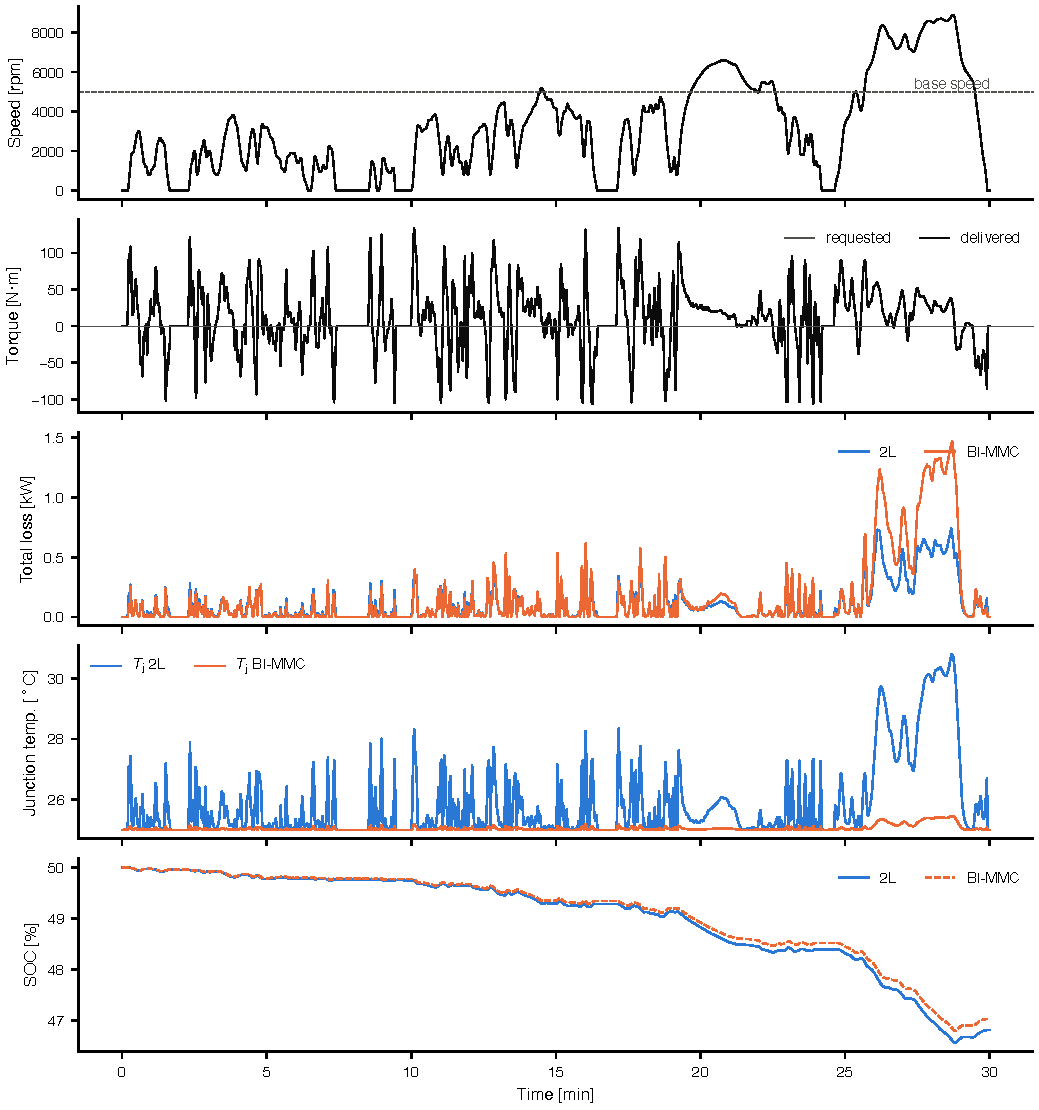
\includegraphics[width=0.9\linewidth]{figures/paper_trace_car.pdf}
\caption{Time series of the passenger car (WLTC, \SI{50}{\percent} initial SOC): machine speed, requested and delivered torque, total loss power, junction temperature, and SOC of both drives.}
\label{fig:trace_car}
\end{figure}

\begin{figure}[ht]
\centering
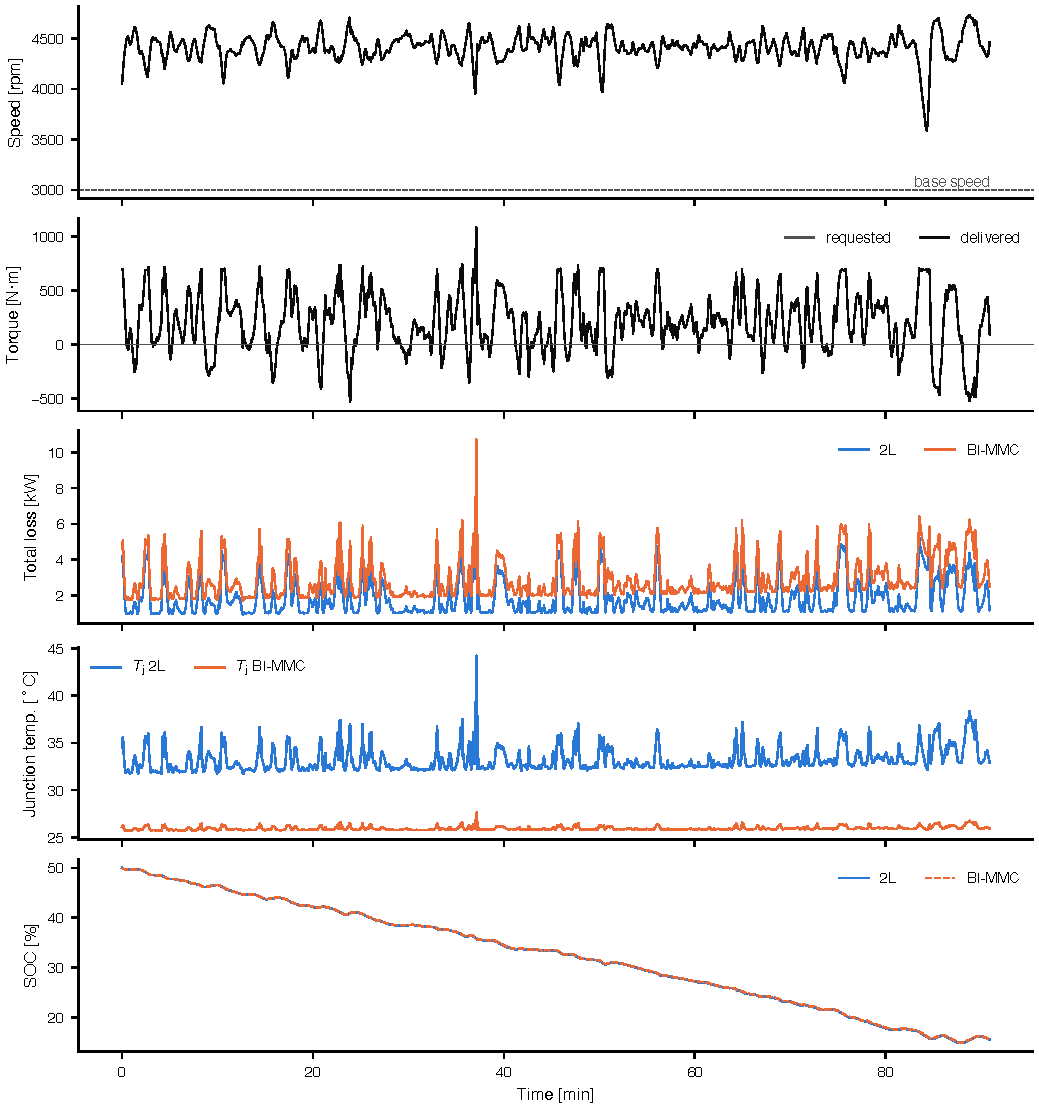
\includegraphics[width=0.9\linewidth]{figures/paper_trace_truck.pdf}
\caption{Time series of the heavy-duty truck (Södertälje--Norrköping, \SI{50}{\percent} initial SOC). The truck stays above base speed on the whole route, which explains the high BI-MMC loss.}
\label{fig:trace_truck}
\end{figure}

\paragraph{Clipped energy.} In the road, off-road and marine cycles, the two drives can deliver the full requested torque (\cref{tab:cycles}). In the synthetic train cycle, the requested regenerative torque (up to \SI{3.8}{\kilo\newton\metre} at the machine) exceeds the base torque of \SI{2.9}{\kilo\newton\metre}, so that the delivered torque differs from the request in \SI{15}{\percent} of the samples, and \SI{11.5}{\kilo\watt\hour} of the \SI{16.1}{\kilo\watt\hour} requested regenerative energy is therefore assigned to the mechanical brake. The train results are thus for a drive that is undersized for the assumed braking, and they should be read with this in mind.

\section{Discussion: Design Rule, Assumptions and Limitations}\label{sec:discussion}
\subsection{Why the cells decide}
The semiconductor advantage of the BI-MMC is large and robust; the battery penalty is what decides the cycle result. At a fixed operating point, both battery losses scale with the inverse of the installed energy. For the 2L pack, with $I_\mathrm{dc}=P/V_\mathrm{dc}$, $V_\mathrm{dc}=N_\mathrm{s}V_\mathrm{cell}$ and $N_\mathrm{p}\approx E_\mathrm{b}/(Q_\mathrm{cell}V_\mathrm{cell}N_\mathrm{s})$, \cref{eq:pb2l} gives
\begin{equation}
P_\mathrm{b}^\mathrm{2L}\approx\frac{(R_0+R_1)\,Q_\mathrm{cell}}{V_\mathrm{cell}}\;\frac{P^2}{E_\mathrm{b}},\qquad \frac{P_\mathrm{b}^\mathrm{2L}}{P}\propto\frac{P}{E_\mathrm{b}},
\label{eq:crate}
\end{equation}
that is, the relative battery loss grows with the C-rate $P/E_\mathrm{b}$ ($Q_\mathrm{cell}$ in Ah, $E_\mathrm{b}$ in Wh). The BI-MMC battery loss follows from \cref{eq:smrc,eq:pbbimmc} with $\Npsm\propto E_\mathrm{b}$ and therefore scales the same way, but with a larger factor because the gated phase current, not the DC current, flows through the cells; the ratio of the two is roughly independent of $E_\mathrm{b}$ at a given point (the cell counts are rounded). The code reproduces this scaling. \Cref{tab:energy} shows the efficiency at one operating point (\SI{0.5}{pu} speed, \SI{0.6}{pu} torque, \SI{50}{\percent} SOC) for halved and doubled energy: the BI-MMC battery loss is $2.0$--$2.7\times$ (car) and about $3\times$ (ship) the 2L loss, but doubling the energy of the passenger car moves the point difference from $-0.45$ to $-0.04$~pp, and the ship's difference becomes positive and grows. This is consistent with the cycle results: the applications with the lowest C-rate (ship \SI{0.4}{\per\hour}, off-road machine \SI{0.75}{\per\hour}) are the ones where the AC battery gains. It suggests a design rule: the AC battery pays off when (i)~most cycle energy is below base speed, so that the cells carry no reactive current, \emph{and} (ii)~the installed energy is large relative to the power, so that the cell losses are small. A systematic sweep of $E_\mathrm{b}$ over complete cycles is a natural use of the platform and is left to future work.

\begin{table}[ht]
\centering
\caption{Point efficiency at \SI{0.5}{pu} speed, \SI{0.6}{pu} torque and \SI{50}{\percent} SOC for different installed energy. $P_\mathrm{b}/E_\mathrm{b}$ is the C-rate of the base power; $P_\mathrm{b}^\mathrm{2L}$, $P_\mathrm{b}^\mathrm{BI}$ here denote the battery loss in W. This is a single operating point and not a cycle result.}
\label{tab:energy}
\footnotesize
\begin{tabular}{@{}lrrrrrrr@{}}
\toprule
Application & $E_\mathrm{b}$ [kWh] & $P_\mathrm{base}/E_\mathrm{b}$ [1/h] & $P_\mathrm{b}^\mathrm{2L}$ [W] & $P_\mathrm{b}^\mathrm{BI}$ [W] & $\eta^\mathrm{2L}$ [\%] & $\eta^\mathrm{BI}$ [\%] & $\Delta\eta$ [pp] \\
\midrule
Passenger car & 38 & 4.00 & 656 & 1338 & 97.58 & 96.71 & -0.88 \\
 & 75 & 2.00 & 328 & 803 & 98.28 & 97.83 & -0.45 \\
 & 150 & 1.00 & 164 & 446 & 98.64 & 98.60 & -0.04 \\
\midrule
Marine vessel & 500 & 0.80 & 360 & 1065 & 98.76 & 98.73 & -0.03 \\
 & 1000 & 0.40 & 180 & 551 & 98.90 & 99.15 & +0.25 \\
 & 2000 & 0.20 & 90 & 275 & 98.98 & 99.38 & +0.40
\\
\bottomrule
\end{tabular}
\end{table}

\subsection{Assumptions and limitations}
The numbers of this paper depend on the following modelling choices, which are fixed in the code and listed so that they can be changed or challenged.
\begin{enumerate}
\item \emph{Scope of the efficiency.} Only converter and battery losses are included. Machine copper, iron and mechanical losses and gear losses (which are only charged to the torque) are not. Because the machine currents of the two drives are almost equal, this should affect the difference less than the absolute values, but a field-weakening current that differs between the drives would change the copper loss.
\item \emph{Conduction model.} Eqs.~\eqref{eq:pc2l} and \eqref{eq:pcbimmc} assume sinusoidal current and equal conduction time of all devices, no body-diode conduction, no dependence on the modulation index and no dead time. The BI-MMC always conducts through two devices per SM.
\item \emph{Switching model.} The switching energy uses the average absolute current $\tfrac2\pi\Ihat$ at a single carrier-period event, constant slopes for the BI-MMC MOSFET (no datasheet curve) and the assumption that all $4\Nsm$ switches of a phase switch once per carrier period. Reverse-recovery, output-capacitance and gate-drive losses are not modelled.
\item \emph{BI-MMC modulation.} All SMs of a phase receive the same gating signal (no phase-shifted carriers, no sorting), and circulating currents, balancing losses and the cost of redundancy beyond the voltage limit are not modelled. The simulation integrates two electrical periods with explicit Euler and a step of $1/(100f_\mathrm{c})$ and requires a speed floor at low speed (\cref{sec:eval}).
\item \emph{2L battery.} The pack loss uses the DC resistance $R_0+R_1$ at the average DC current. The DC-link ripple current and capacitor losses are neglected.
\item \emph{Thermal.} Junction, case and cell temperatures are steady-state values with fixed thermal resistances, no thermal capacitance and a constant coolant temperature. $\Rds(\Tj)$ is the only coupling to the losses. Cell aging, SOC dependence of the thermal path and temperature dependence of the cell resistance are not modelled.
\item \emph{Control.} Currents are MTPA with voltage-limited field weakening at the OCV of the present SOC, the modulation limit is $V_\mathrm{dc}/\sqrt3$ for the 2L and $\Nssm\Nsm V_\mathrm{cell}$ for the BI-MMC, and no voltage margin or current-control dynamics are included. The 2L carrier frequency is fixed at \SI{10}{\kilo\hertz} for all speeds.
\item \emph{Sizing and fairness.} Both drives get the same cell type and energy up to the rounding of the cell counts (the BI-MMC has $-0.8$ to $+8.4$~\% cells relative to the 2L pack, \cref{tab:conv}), and the BI-MMC string voltage is up to \SI{4.1}{\percent} above the 2L limit. The number of series cells per SM is an input, set per application; the default of 10 would give the car \SI{20}{\percent} more cells. Design choices that favour one side, such as the pulse number $m_\mathrm{f}=2$, the number of parallel devices, or the SM count, are inputs and are not optimised. The rated power and gear ratios of the bus, truck and train were sized so that the cycles stay inside the torque and power limits.
\item \emph{Quasi-static evaluation.} Each cycle sample (mostly \SI{1}{\second}) is evaluated at steady state; faster transients are not captured. The common torque is the minimum of both drives, and in the synthetic train cycle part of the braking energy is clipped.
\item \emph{Data.} The vehicle parameters are typical values, the truck road and vehicle data originate from an earlier truck study (files in \code{so_no/}) whose provenance still has to be documented, and the cell parameters are a nominal 24~Ah NMC cell with SOC scaling polynomials. The cycle results are therefore indicative of trends.
\end{enumerate}

\subsection{Sensitivity analysis and further use}
\code{sens.py} sweeps every user input one at a time by $\pm30\,\%$ (integer parameters are rounded, SOC and redundancy use absolute ranges) around the nominal values and records the point efficiency of both drives at a chosen speed and torque, producing a table and a tornado chart. It uses the same \code{model.loss_maps} as the other analyses. The same dictionary-based interface allows a sweep over complete cycles with \code{cycle_eval.evaluate_cycle}.

\section{Conclusion}
This paper has documented an open-source evaluation platform for comparing a two-level SiC inverter with an AC battery (BI-MMC) in two analyses that share every loss equation: torque--speed efficiency maps, and drive-cycle efficiency with SOC and temperature tracking. All equations of the Python implementation, the algorithms of both analyses and their assumptions are given.

Applied to six applications with equal machine, cells and installed energy, the platform shows that the AC battery cuts the semiconductor loss energy by \SIrange{26}{80}{\percent} but increases the battery loss energy by a factor of \numrange{1.6}{4.4}, because the cells carry the switched phase current. On a cycle basis, the AC battery is therefore at best marginally better (\SI{+0.09}{\pp} for the off-road machine and \SI{+0.10}{\pp} for the ship, where nearly all energy is delivered below base speed and the installed energy is large relative to the power) and clearly worse for the passenger car and city bus ($-0.49$ and $-0.57$~pp), the long-haul truck ($-0.83$~pp) and the regional train ($-1.74$~pp). Low SOC aggravates the losses of the AC battery. The answer to the title question is thus: only in low-speed, low-C-rate duty, and then by only about \SI{0.1}{\pp}.

The platform also shows which levers could change this answer: a higher installed energy per unit power, a lower cell resistance, a smaller field-weakening current, and a modulation that reduces the cell current. The platform, the application presets, the data files and the scripts that generate every figure and table of this paper are provided in the repository, so that the study can be repeated with other machines, cells, devices and duty cycles.


\printbibliography

\appendix
\section{Parameters and Data}\label{app:params}
\Cref{tab:params} lists every entry of the parameter dictionary \code{model.NOMINAL} with the default value. The application presets override \code{PBase}, \code{wmBase}, \code{Vdc} and \code{Ebatt} (\cref{tab:machine}), and the car also \code{Nscells_b}. \Cref{tab:ocv} lists the open-circuit voltage tables, and \cref{tab:rdsonpoly} the Rdson polynomials.

\begin{longtable}{@{}p{3.3cm}p{2.5cm}p{2.0cm}p{8.4cm}@{}}
\caption{User-input dictionary \code{model.NOMINAL}.}\label{tab:params}\\
\toprule
Key & Default & Unit & Meaning \\
\midrule
\endfirsthead
\toprule
Key & Default & Unit & Meaning \\
\midrule
\endhead
\multicolumn{4}{@{}l}{\emph{general}} \\
\code{soc} & 0.5 & -- & operating SOC (sensitivity analysis) \\
\multicolumn{4}{@{}l}{\emph{PMSM}} \\
\code{pp} & 4 & -- & pole pairs $p$ \\
\code{PBase} & 400\,000 & W & base power $P_\mathrm{b}$ \\
\code{wmBase} & 3000 & rpm & base speed $n_\mathrm{b}$ \\
\code{Vdc} & 700 & V & DC-link voltage $V_\mathrm{dc}$ \\
\code{rs_pu}, \code{ld_pu}, \code{lq_pu} & 0.01, 0.55, 0.85 & pu & stator resistance, d- and q-axis inductance \\
\multicolumn{4}{@{}l}{\emph{two-level inverter}} \\
\code{mosfet} & "Wolfspeed" & -- & device data set ("Wolfspeed" or "custom") \\
\code{fsw} & 10\,000 & Hz & carrier frequency $f_\mathrm{sw}$ \\
\code{Rdson_2l} & 4.6\,m$\Omega$ & \si{\ohm} & on-resistance at \SI{25}{\celsius} (datasheet) \\
\code{ImosRated_RMS} & 320 & A (RMS) & device current rating (sets $N_\mathrm{p,mos}$) \\
\code{Rth_jc_2l}, \code{Rth_ca_2l} & 0.08, 0.05 & K/W & junction-to-case, case-to-ambient \\
\code{Tjmax_2l}, \code{Tcmax_2l} & 175, 100 & \si{\celsius} & thermal limits (reported, not enforced) \\
\code{Tambient} & 25 & \si{\celsius} & ambient (coolant) temperature \\
\code{didt_on_2l}, \dots, \code{dvdt_off_2l} & 8, 15, 25, 25 & A/ns, V/ns & switching slopes, only for the custom device \\
\multicolumn{4}{@{}l}{\emph{battery}} \\
\code{chemistry} & "NMC" & -- & OCV table (NMC, LFP, LTO, NaB) \\
\code{Ebatt} & 400\,000 & Wh & installed energy $E_\mathrm{b}$ \\
\code{Qcell} & 24 & Ah & cell capacity \\
\code{R0_nom}, \code{R1_nom} & 1.2, 0.7 & m$\Omega$ & nominal cell resistances \\
\code{poly_r}, \code{poly_c} & (1.3,$-$1.3,1.3), ($-$1.3,1.3,1.3) & -- & SOC scaling polynomials $[a_2,a_1,a_0]$ of $R_0,R_1$ and $C_1$ \\
\code{C1_nom} & $1/(2\pi\cdot250\,R_1)$ & F & optional; default gives a \SI{250}{\hertz} RC corner \\
\code{lz_cell}, \code{kz_cell}, \code{Az_cell} & 0.027, 25, 0.003996 & m, W/mK, m$^2$ & cell thermal path (bottom cooled) \\
\multicolumn{4}{@{}l}{\emph{BI-MMC}} \\
\code{Nscells_b} & 10 & -- & series cells per submodule $\Nssm$ (input); $\Nsm$ follows \\
\code{Nsm_redundant_pu} & 0 & pu & redundant SM share $r$ \\
\code{Rdson_bimmc} & 0.3 & m$\Omega$ & on-resistance at \SI{25}{\celsius} \\
\code{Rdson_poly_bimmc} & None & -- & optional cubic $[c_3..c_0]$; None uses the datasheet fit \\
\code{Imax_mosfet} & 400 & A (RMS) & device rating (sets $N_\mathrm{p,mos}$, at least 4) \\
\code{didt_on_bimmc}, \code{didt_off_bimmc} & 1, 1 & A/ns & constant switching slopes \\
\code{dvdt_on_bimmc}, \code{dvdt_off_bimmc} & 0.5, 0.5 & V/ns & constant switching slopes \\
\code{mf_bimmc} & 2 & -- & pulse number $m_\mathrm{f}$ ($f_\mathrm{c}=m_\mathrm{f}f_\mathrm{e}$) \\
\code{Rth_jc_bimmc}, \code{Rth_ca_bimmc} & 0.5, 0.2 & K/W & junction-to-case, case-to-ambient \\
\code{Tjmax_bimmc} & 175 & \si{\celsius} & junction limit (reported, not enforced) \\
\bottomrule
\end{longtable}

\begin{table}[ht]
\centering
\caption{Cell open-circuit voltage [V] versus SOC (\code{model.OCV}); linear interpolation in between.}
\label{tab:ocv}
\footnotesize
\setlength\tabcolsep{3pt}
\begin{tabular}{@{}lrrrrrrrrrrr@{}}
\toprule
SOC & 1.0 & 0.9 & 0.8 & 0.7 & 0.6 & 0.5 & 0.4 & 0.3 & 0.2 & 0.1 & 0.0 \\
\midrule
NMC & 4.13 & 4.03 & 3.92 & 3.83 & 3.75 & 3.70 & 3.66 & 3.63 & 3.59 & 3.53 & 3.34 \\
LFP & 3.39 & 3.33 & 3.31 & 3.32 & 3.31 & 3.29 & 3.27 & 3.26 & 3.25 & 3.18 & 2.89 \\
LTO & 2.69 & 2.42 & 2.35 & 2.32 & 2.28 & 2.23 & 2.20 & 2.19 & 2.18 & 2.15 & 2.11 \\
NaB & 3.90 & 3.74 & 3.61 & 3.47 & 3.29 & 3.12 & 2.99 & 2.87 & 2.75 & 2.55 & 2.22 \\
\bottomrule
\end{tabular}
\end{table}

\begin{table}[ht]
\centering
\caption{Cubic polynomials $\rho(\Tj)=c_3\Tj^3+c_2\Tj^2+c_1\Tj+c_0$ (\si{\celsius}); the code divides by $\rho(25)$. The Wolfspeed polynomial is the default of the custom device (\code{RDSON_POLY_DEFAULT}); for the Wolfspeed module the code re-fits the datasheet points at run time. The Infineon polynomial is \code{RDSON_POLY_BIMMC_DATASHEET}, also produced by \code{fit_rdson.py}.}
\label{tab:rdsonpoly}
\footnotesize
\begin{tabular}{@{}lrrrr@{}}
\toprule
 & $c_3$ & $c_2$ & $c_1$ & $c_0$ \\
\midrule
Wolfspeed (default of custom) & $9.4346\times10^{-12}$ & $2.9952\times10^{-5}$ & $5.7710\times10^{-4}$ & $0.96766$ \\
Infineon IQDH29NE2LM5CGSC & $1.2594\times10^{-8}$ & $5.4270\times10^{-6}$ & $3.0254\times10^{-3}$ & $0.92114$ \\
\bottomrule
\end{tabular}
\end{table}

\paragraph{Datasheet data.} The folder \code{data/} holds the digitised datasheet curves: switching slopes versus device current of the Wolfspeed module (\code{Wolfspeed_MOSFET_dvdt_didt_data.csv}, four curves with their own current axes), normalised $\Rds(\Tj)$ of the Wolfspeed module and of the Infineon device (two CSV files), and the duty cycles in \code{data/cycles/} with a README that records source, regulation, transformations and cross-checks of every file.

\section{Function Reference}\label{app:reference}
This appendix lists the public functions of the package with their arguments, their results and the equation they implement. Units are SI unless stated.

\subsection*{calc.py}
\begin{description}\itemsep0pt
\item[\code{MotorParameters}, \code{SwitchingSlopes}, \code{BatteryParameters}, \code{ThermalParameters}] Frozen dataclasses for the machine (\code{stator_resistance}, \code{d_axis_inductance}, \code{q_axis_inductance}, \code{magnet_flux}, \code{pole_pairs}), the slopes (constants or functions of the device current in A/ns, V/ns, floored at $10^{-6}$ to avoid a division by zero), the cell equivalent circuit ($R_0$, $R_1$, $C_1$, series and parallel cells), and the thermal network (ambient, $R_\mathrm{th,jc}$, $R_\mathrm{th,ca}$).
\item[\code{TwoLevelLossConfig}, \code{BimmcLossConfig}] Configuration of the two loss functions: DC or SM voltage, on-resistance, parallel devices, switching frequency (scalar or array for the BI-MMC), battery, thermal network, slopes; the BI-MMC additionally has the SM count, redundancy, pole pairs, an optional $\rho(\Tj)$ function and the number of fixed-point steps.
\item[\code{create_mtpa_optimization_problem(motor)}] Builds the CasADi \code{Opti} problem of \cref{eq:mtpa}; returns \code{(opti, x, (Tau_ref, wm_ref, vmax))}, with the three parameters set by the caller. Solver: IPOPT, print level 0.
\item[\code{calc_losses_2l(Id, Iq, Vd, Vq, config)}] \cref{eq:pc2l,eq:times,eq:ps2l,eq:thermal2l,eq:pb2l}; arrays or scalars; returns \code{(Pmos_loss, Psw_loss, Pbatt, Tj, Tc)} in W and \si{\celsius}.
\item[\code{calc_losses_bimmc(Id, Iq, Vd, Vq, wm_ref, Te_ref, config)}] \cref{eq:pcbimmc,eq:psbimmc,eq:io,eq:vref,eq:gate,eq:ib,eq:smrc,eq:rcsim,eq:pbbimmc} on a (speed $\times$ torque) array; \code{wm_ref} is the mechanical speed vector, \code{Te_ref} the torque vector (only its length is used). Rows with $\omega_\mathrm{e}\le0$ and NaN points return NaN battery loss. Returns the same five outputs.
\item[\code{batterymdel(ib, R0, R1, C1, Vc)}, \code{simulate_battery_loss(ib_profile, tvec, R0, R1, C1, t_avg_start)}] Numba-compiled right-hand side of \cref{eq:rcsim} and the explicit-Euler integration; the average loss is taken for $t\ge t_\mathrm{avg,start}$.
\end{description}

\subsection*{model.py}
\begin{description}\itemsep0pt
\item[\code{NOMINAL}, \code{OCV}] Default inputs (\cref{tab:params}) and OCV tables (\cref{tab:ocv}).
\item[\code{design(p)} $\to$ \code{Design}] \cref{eq:base1,eq:base2,eq:base3,eq:wmax,eq:pack2l,eq:npsm} and the parallel device counts; raises \code{ValueError} if $L_\mathrm{d}I_\mathrm{b}\ge\psi_\mathrm{f}$.
\item[\code{cell_state(p, soc)}] Returns $(V_\mathrm{cell},R_0,R_1,C_1)$ of \cref{eq:cellrc}; accepts arrays for SOC.
\item[\code{cell_rth(p)}, \code{cell_temperature(p, Pbatt, n_cells)}] \cref{eq:tcell}.
\item[\code{mosfet_raw(p)}, \code{mosfet_data(p)}, \code{bimmc_rdson_raw()}, \code{bimmc_rdson_fun(p)}] Datasheet tables and the interpolation functions of the slopes and the normalised $\Rds(\Tj)$ (\code{rdson_poly_fun}, \code{fit_rdson_poly}).
\item[\code{solve_mtpa(d, vmax, wm_vec, T_vec, PBase)}] MTPA currents on the grid, NaN for infeasible points (\cref{sec:mtpa}).
\item[\code{dq_voltages(d, Id, Iq, wm_vec)}] \cref{eq:vd,eq:vq}.
\item[\code{loss_maps(p, soc, wm_vec, T_vec, voltage_limit, rdson_tj, rdson_iter)}] \Cref{alg:maps}; returns a dictionary with the grid, the voltage limits, currents, $P_\mathrm{c}$, $P_\mathrm{s}$, $P_\mathrm{b}$, $\Tj$, $\Tc$, $T_\mathrm{cell}$ and the thermal-limit flags of both drives.
\item[\code{efficiency(Pout, Ploss)}, \code{default_grid(p, n_speed, n_torque)}] \cref{eq:eta} and the default 50$\times$100 grid.
\end{description}

\subsection*{applications.py and cycles.py}
\begin{description}\itemsep0pt
\item[\code{APPLICATIONS}] Dictionary of the six presets (\code{params}, \code{vehicle}, \code{cycle}, \code{label}); \code{E3_MODES} holds the ISO 8178 E3 table.
\item[\code{road_load_force(veh, v, a, slope)}, \code{gear_ratio(app)}] \cref{eq:roadload,eq:resistance} and the gear ratio of \cref{sec:profile}.
\item[\code{machine_profile(app)}] Dispatches to \code{speed_cycle}, \code{road_cycle} (\cref{eq:cruise}), \code{normalised_cycle} (\cref{eq:nrtc}), \code{mode_cycle} and \code{rail_cycle} (\cref{eq:rail}); returns \code{t}, \code{dt}, \code{v}, \code{wm}, \code{T} (and \code{slope} for road cycles).
\end{description}

\subsection*{cycle\_eval.py}
\begin{description}\itemsep0pt
\item[\code{make_mtpa_solver(d)}, \code{mtpa_point(solver, d, wm, T, vmax)}] Reusable MTPA problem with warm start; returns $(i_\mathrm{d},i_\mathrm{q})$ or None if infeasible.
\item[\code{feasible_torque(solver, d, wm, T_req, vmax)}] Largest feasible torque with ten bisection steps (\cref{eq:bisect}); returns \code{(T, (Id, Iq))}.
\item[\code{losses_2l(...)}, \code{losses_bimmc(...)}] Single-point wrappers around \code{calc.calc_losses_2l} and \code{calc.calc_losses_bimmc}, including the $\Rds$ iteration and the BI-MMC speed floor.
\item[\code{evaluate_cycle(app_key, soc0, rdson_iter=5)}] \Cref{alg:cycle}; returns the summary dictionary (\cref{sec:metrics}) and the per-sample trace.
\item[\code{compute_maps(app_key, soc, n_speed, n_torque)}] Cached loss maps (NPZ in \code{results_cycles/}), used for the map backgrounds of the cycle figures.
\item[\code{main()}] Command line: \code{--apps}, \code{--soc}, \code{--jobs}; writes the JSON, the Excel table and one CSV per job.
\end{description}

\subsection*{Front ends and utilities}
\begin{description}\itemsep0pt
\item[\code{main.py}] Streamlit dashboard: sidebar inputs (machine, device, battery, BI-MMC) $\to$ parameter dictionary $\to$ \code{model.loss_maps} $\to$ tabs for parameters, MTPA maps, loss and efficiency maps, comparison; saves figures and one Excel workbook.
\item[\code{create_maps_PCIM.py}] \code{create_maps(app_key, soc, out_dir, xlsx)} produces the figure set of Analysis~I for an application; constants \code{VOLTAGE_LIMIT} and \code{RDSON_TJ} select the settings.
\item[\code{plots.py}, \code{export.py}] \code{plot_*} functions for the data classes of \cref{sec:maps}; \code{write_workbook} writes maps as torque $\times$ speed blocks.
\item[\code{sens.py}] \code{evaluate(p, speed_pu, torque_pu)} returns the point efficiencies of both drives; \code{run_sensitivity} sweeps the parameters of the list \code{SWEPT}; \code{plot_results} draws the sweep and tornado charts.
\item[\code{fit_rdson.py}] Least-squares polynomial of degrees 1 to 5, RMSE and the equation string for the Infineon data.
\end{description}

\section{Output Formats}\label{app:outputs}
\paragraph{Cycle summary} (\code{results_cycles/cycle_results.json}, \code{.xlsx}): one record per application and initial SOC, with
\code{app}, \code{label}, \code{cycle}, \code{soc_start}, \code{soc_end_2l}, \code{soc_end_bimmc}, \code{duration_s}, \code{distance_km}, \code{E_motoring_kWh}, \code{E_regen_kWh}, \code{E_clipped_motoring_kWh}, \code{E_clipped_regen_kWh}, \code{n_infeasible}, \code{share_below_base_speed}, \code{gear_ratio}, and for each drive $X\in\{$\code{2l}, \code{bimmc}$\}$: \code{E_Pc_X_kWh}, \code{E_Ps_X_kWh}, \code{E_Pb_X_kWh}, \code{E_loss_X_kWh}, \code{Tj_max_X}, \code{Tc_max_X}, \code{Tcell_max_X}, \code{eta_cycle_X}, \code{E_batt_net_X_kWh}, \code{kWh_per_100km_X}; and \code{delta_eta_pp}, \code{delta_loss_pct}.

\paragraph{Cycle trace} (\code{results_cycles/losses_<app>_soc<NN>.csv}): one row per sample with \code{t}, \code{wm} [rad/s], \code{T_req}, \code{dt}, \code{soc_2l}, \code{soc_bimmc}, \code{T} (delivered), \code{P}, \code{infeasible}, and for each drive \code{Pc}, \code{Ps}, \code{Pb}, \code{Tj}, \code{Tc}, \code{Ploss}, \code{Tcell} with the suffix \code{_2l} or \code{_bimmc}.

\paragraph{Map workbook} (\code{plot_data_*.xlsx}): sheets \code{Parameters}, the datasheet data and fits (\code{Switching_slopes_data}, \code{Switching_slopes_fit}, \code{Rdson_2L}, \code{Rdson_BIMMC}), the cell data (\code{Cell_OCV}, \code{Cell_RC_parameters}), and the maps of the MTPA analysis and of both converters and their comparison, each as one block per quantity with torque in rows and speed in columns; empty cells are infeasible or not plotted points.

\paragraph{Figures} (\code{<out>/<application>/*.png}): \code{mtpa_maps}, \code{mtpa_maps_dqs}, \code{losses_maps_{2l,bimmc,comparison}}, \code{temperature_maps_{2l,bimmc}}, \code{efficiency_maps_{2l,bimmc,comparison}}, \code{individual_losses_maps_comparison} and \code{individual_efficiency_maps_comparison}, each with the suffix \code{_soc_<NN>}.

\paragraph{Reproducing this paper.}
\begin{lstlisting}[numbers=none, language={}]
python/venv/bin/python python/cycle_eval.py --soc 0.2 0.5 0.9
python/venv/bin/python doc/figures/make_cycle_figures.py
python/venv/bin/python doc/figures/make_paper_maps.py
python/venv/bin/python doc/figures/make_paper_assets.py
cd doc && latexmk -pdf PCIM_paper.tex
\end{lstlisting}

\section{Additional Results}\label{app:traces}
\subsection*{Cycle results for all initial SOC values}
\begin{table}[H]
\centering
\caption{Loss energies in kWh (conduction, switching, battery) and cycle efficiency of both drives for initial SOC of \SIlist{20;50;90}{\percent}.}
\label{tab:resfull}
\footnotesize
\setlength\tabcolsep{3pt}
\begin{tabular}{@{}lrrrrrrrrrr@{}}
\toprule
 & & \multicolumn{3}{c}{2L [kWh]} & \multicolumn{3}{c}{BI-MMC [kWh]} & \multicolumn{2}{c}{$\etacyc$ [\%]} & \\
Application & SOC [\%] & $E_\mathrm{c}$ & $E_\mathrm{s}$ & $E_\mathrm{b}$ & $E_\mathrm{c}$ & $E_\mathrm{s}$ & $E_\mathrm{b}$ & 2L & BI & $\Delta\etacyc$ [pp] \\
\midrule
Passenger car & 20 & 0.024 & 0.018 & 0.019 & 0.014 & 0.004 & 0.081 & 98.75 & 97.98 & -0.77 \\
 & 50 & 0.021 & 0.018 & 0.015 & 0.012 & 0.003 & 0.063 & 98.87 & 98.38 & -0.49 \\
 & 90 & 0.016 & 0.018 & 0.015 & 0.010 & 0.003 & 0.055 & 98.97 & 98.62 & -0.34 \\
\midrule
City bus & 20 & 0.165 & 0.137 & 0.101 & 0.114 & 0.025 & 0.458 & 98.21 & 97.35 & -0.86 \\
 & 50 & 0.150 & 0.137 & 0.084 & 0.104 & 0.024 & 0.373 & 98.35 & 97.78 & -0.57 \\
 & 90 & 0.114 & 0.136 & 0.086 & 0.079 & 0.022 & 0.344 & 98.51 & 98.02 & -0.48 \\
\midrule
Heavy-duty truck & 20 & 1.148 & 0.928 & 1.513 & 1.197 & 0.228 & 5.071 & 98.05 & 96.47 & -1.58 \\
 & 50 & 0.846 & 0.878 & 1.115 & 0.882 & 0.197 & 3.289 & 98.45 & 97.62 & -0.83 \\
 & 90 & 0.577 & 0.806 & 1.001 & 0.600 & 0.161 & 2.509 & 98.70 & 98.22 & -0.48 \\
\midrule
Off-road machine & 20 & 0.042 & 0.044 & 0.099 & 0.015 & 0.002 & 0.165 & 98.92 & 98.94 & +0.02 \\
 & 50 & 0.042 & 0.046 & 0.081 & 0.015 & 0.003 & 0.137 & 99.02 & 99.10 & +0.09 \\
 & 90 & 0.042 & 0.053 & 0.081 & 0.015 & 0.003 & 0.144 & 98.98 & 99.06 & +0.08 \\
\midrule
Marine vessel & 20 & 0.772 & 0.637 & 1.083 & 0.626 & 0.050 & 1.692 & 98.99 & 99.04 & +0.05 \\
 & 50 & 0.772 & 0.682 & 0.862 & 0.626 & 0.053 & 1.385 & 99.06 & 99.17 & +0.10 \\
 & 90 & 0.775 & 0.768 & 0.852 & 0.626 & 0.060 & 1.448 & 99.03 & 99.14 & +0.11 \\
\midrule
Regional train & 20 & 0.446 & 0.293 & 1.398 & 0.503 & 0.061 & 3.080 & 96.68 & 94.34 & -2.34 \\
 & 50 & 0.418 & 0.300 & 1.141 & 0.471 & 0.061 & 2.463 & 97.15 & 95.40 & -1.74 \\
 & 90 & 0.365 & 0.314 & 1.133 & 0.411 & 0.058 & 2.444 & 97.23 & 95.54 & -1.68
\\
\bottomrule
\end{tabular}
\end{table}

\begin{figure}[H]
\centering
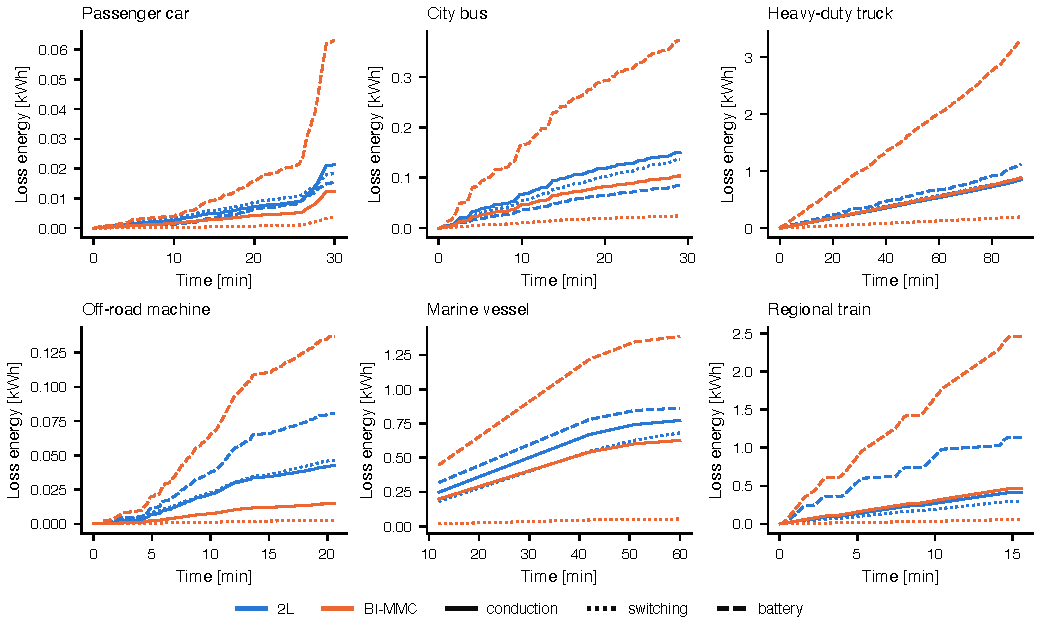
\includegraphics[width=\linewidth]{figures/paper_loss_energy.pdf}
\caption{Cumulative loss energy along each cycle (\SI{50}{\percent} initial SOC): conduction (solid), switching (dotted) and battery (dashed) loss of the 2L inverter (blue) and the BI-MMC (orange).}
\label{fig:lossenergy}
\end{figure}

\subsection*{Time series}
\begin{figure}[H]
\centering
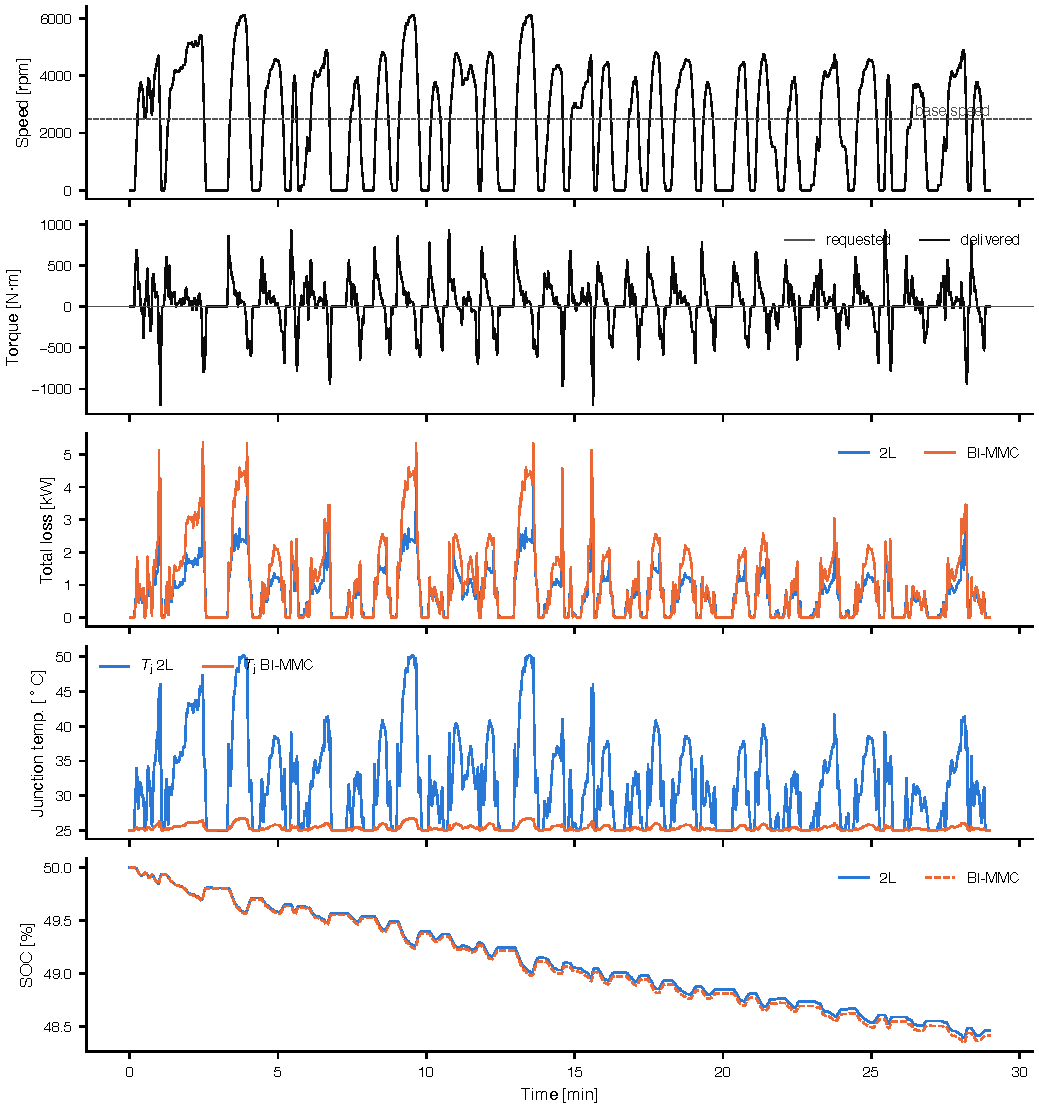
\includegraphics[width=0.88\linewidth]{figures/paper_trace_bus.pdf}
\caption{Time series of the city bus (Braunschweig, \SI{50}{\percent} initial SOC). The speed spikes above base speed are short, but the regenerative torque peaks are large.}
\end{figure}
\begin{figure}[H]
\centering
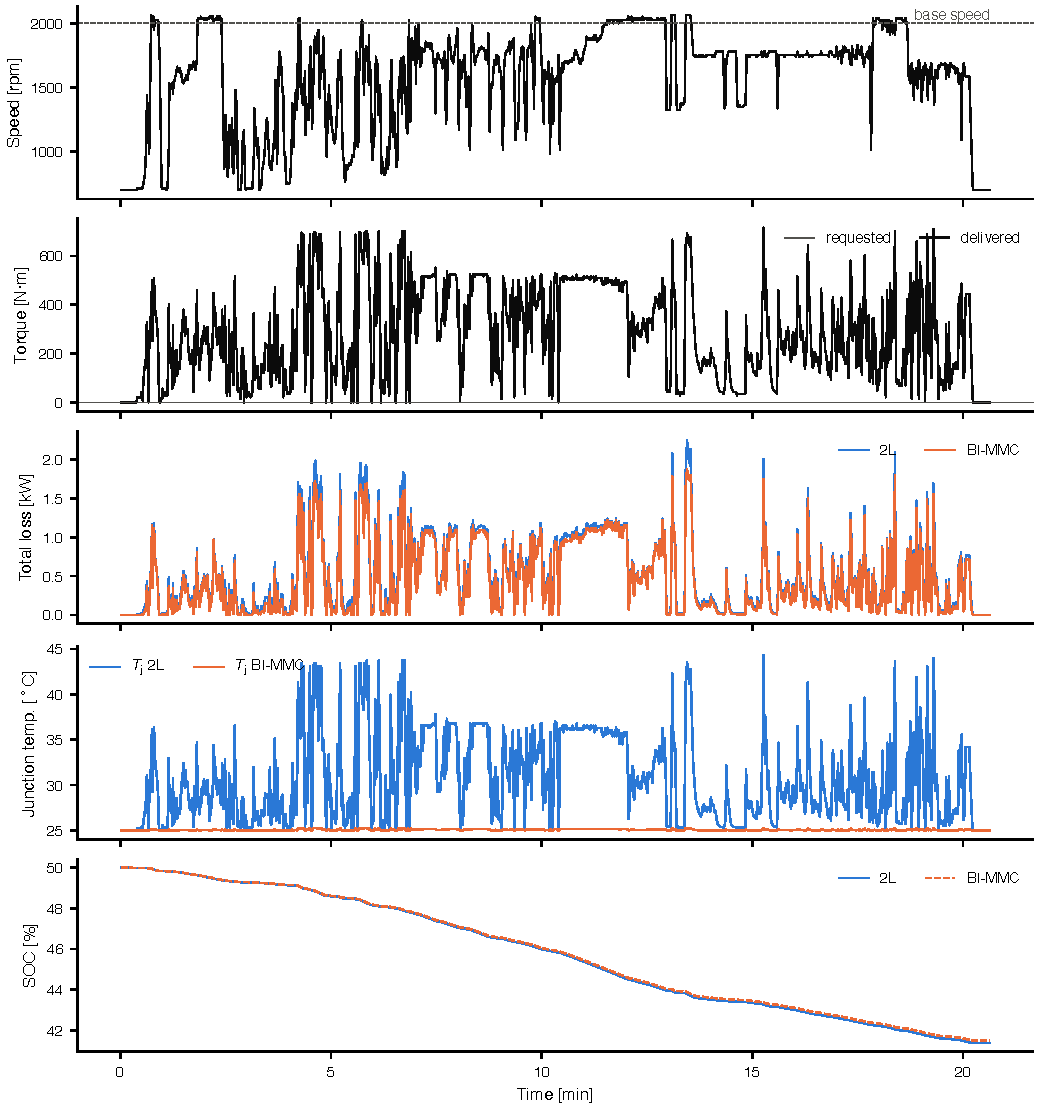
\includegraphics[width=0.88\linewidth]{figures/paper_trace_offroad.pdf}
\caption{Time series of the off-road machine (NRTC, \SI{50}{\percent} initial SOC).}
\end{figure}
\begin{figure}[H]
\centering
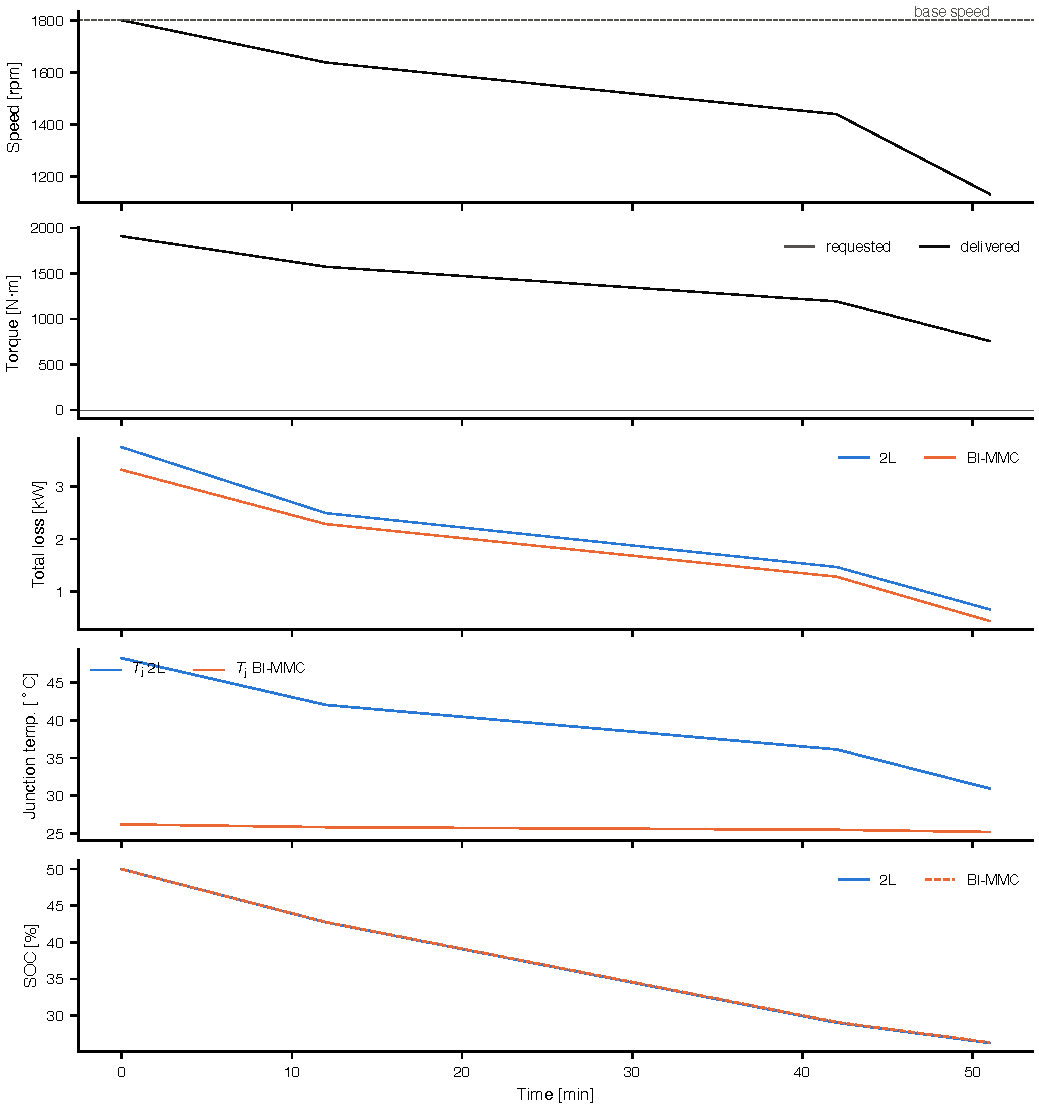
\includegraphics[width=0.88\linewidth]{figures/paper_trace_marine.pdf}
\caption{Time series of the marine vessel (ISO 8178 E3 modes, \SI{50}{\percent} initial SOC): four steady modes.}
\end{figure}
\begin{figure}[H]
\centering
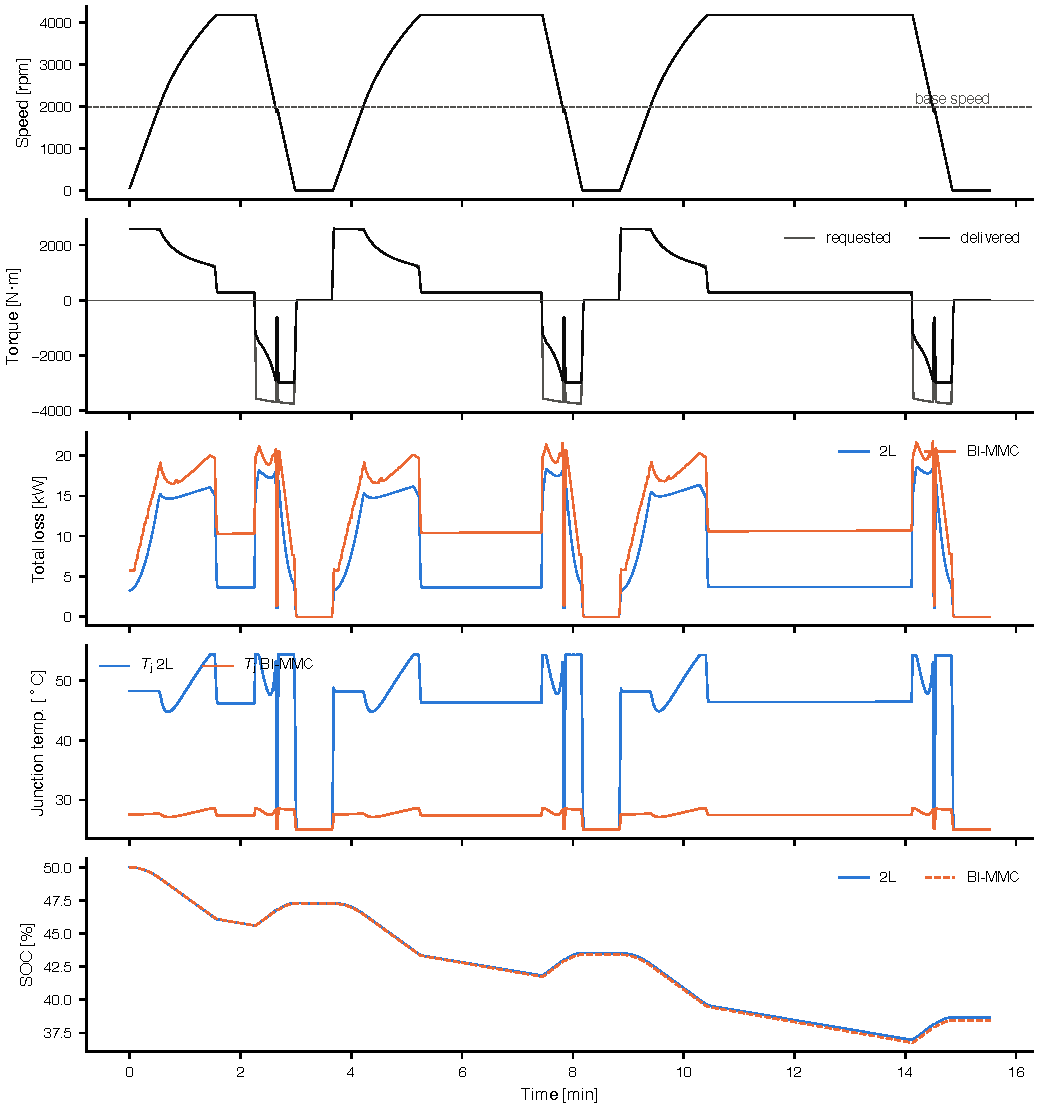
\includegraphics[width=0.88\linewidth]{figures/paper_trace_train.pdf}
\caption{Time series of the regional train (synthetic run, \SI{50}{\percent} initial SOC). The requested regenerative torque exceeds the torque limit, so the delivered torque is lower.}
\end{figure}

\subsection*{Efficiency maps of the remaining applications}
\begin{figure}[H]
\centering
\includegraphics[width=0.49\linewidth]{figures/maps/bus/efficiency_maps_comparison_soc_50.png}\hfill
\includegraphics[width=0.49\linewidth]{figures/maps/marine/efficiency_maps_comparison_soc_50.png}
\caption{Efficiency of the 2L inverter, the BI-MMC and their difference at \SI{50}{\percent} SOC for the city bus (left) and the marine vessel (right).}
\end{figure}
\begin{figure}[H]
\centering
\includegraphics[width=0.49\linewidth]{figures/maps/train/efficiency_maps_comparison_soc_50.png}\hfill
\includegraphics[width=0.49\linewidth]{figures/maps/train/losses_maps_comparison_soc_50.png}
\caption{Regional train at \SI{50}{\percent} SOC: efficiency of both drives and their difference (left), and total losses of both drives and their difference (right).}
\end{figure}


\end{document}
